\documentclass[]{article}
\usepackage{lmodern}
\usepackage{amssymb,amsmath}
\usepackage{ifxetex,ifluatex}
\usepackage{fixltx2e} % provides \textsubscript
\ifnum 0\ifxetex 1\fi\ifluatex 1\fi=0 % if pdftex
  \usepackage[T1]{fontenc}
  \usepackage[utf8]{inputenc}
\else % if luatex or xelatex
  \ifxetex
    \usepackage{mathspec}
  \else
    \usepackage{fontspec}
  \fi
  \defaultfontfeatures{Ligatures=TeX,Scale=MatchLowercase}
\fi
% use upquote if available, for straight quotes in verbatim environments
\IfFileExists{upquote.sty}{\usepackage{upquote}}{}
% use microtype if available
\IfFileExists{microtype.sty}{%
\usepackage{microtype}
\UseMicrotypeSet[protrusion]{basicmath} % disable protrusion for tt fonts
}{}
\usepackage[margin=1in]{geometry}
\usepackage{hyperref}
\hypersetup{unicode=true,
            pdftitle={Zur Wahrnehmung und Einstellung von WU-Studierenden gegenüber Fremden},
            pdfauthor={Boris Podzeit, Yasir Khan},
            pdfborder={0 0 0},
            breaklinks=true}
\urlstyle{same}  % don't use monospace font for urls
\usepackage{natbib}
\bibliographystyle{plainnat}
\usepackage{color}
\usepackage{fancyvrb}
\newcommand{\VerbBar}{|}
\newcommand{\VERB}{\Verb[commandchars=\\\{\}]}
\DefineVerbatimEnvironment{Highlighting}{Verbatim}{commandchars=\\\{\}}
% Add ',fontsize=\small' for more characters per line
\usepackage{framed}
\definecolor{shadecolor}{RGB}{248,248,248}
\newenvironment{Shaded}{\begin{snugshade}}{\end{snugshade}}
\newcommand{\KeywordTok}[1]{\textcolor[rgb]{0.13,0.29,0.53}{\textbf{{#1}}}}
\newcommand{\DataTypeTok}[1]{\textcolor[rgb]{0.13,0.29,0.53}{{#1}}}
\newcommand{\DecValTok}[1]{\textcolor[rgb]{0.00,0.00,0.81}{{#1}}}
\newcommand{\BaseNTok}[1]{\textcolor[rgb]{0.00,0.00,0.81}{{#1}}}
\newcommand{\FloatTok}[1]{\textcolor[rgb]{0.00,0.00,0.81}{{#1}}}
\newcommand{\ConstantTok}[1]{\textcolor[rgb]{0.00,0.00,0.00}{{#1}}}
\newcommand{\CharTok}[1]{\textcolor[rgb]{0.31,0.60,0.02}{{#1}}}
\newcommand{\SpecialCharTok}[1]{\textcolor[rgb]{0.00,0.00,0.00}{{#1}}}
\newcommand{\StringTok}[1]{\textcolor[rgb]{0.31,0.60,0.02}{{#1}}}
\newcommand{\VerbatimStringTok}[1]{\textcolor[rgb]{0.31,0.60,0.02}{{#1}}}
\newcommand{\SpecialStringTok}[1]{\textcolor[rgb]{0.31,0.60,0.02}{{#1}}}
\newcommand{\ImportTok}[1]{{#1}}
\newcommand{\CommentTok}[1]{\textcolor[rgb]{0.56,0.35,0.01}{\textit{{#1}}}}
\newcommand{\DocumentationTok}[1]{\textcolor[rgb]{0.56,0.35,0.01}{\textbf{\textit{{#1}}}}}
\newcommand{\AnnotationTok}[1]{\textcolor[rgb]{0.56,0.35,0.01}{\textbf{\textit{{#1}}}}}
\newcommand{\CommentVarTok}[1]{\textcolor[rgb]{0.56,0.35,0.01}{\textbf{\textit{{#1}}}}}
\newcommand{\OtherTok}[1]{\textcolor[rgb]{0.56,0.35,0.01}{{#1}}}
\newcommand{\FunctionTok}[1]{\textcolor[rgb]{0.00,0.00,0.00}{{#1}}}
\newcommand{\VariableTok}[1]{\textcolor[rgb]{0.00,0.00,0.00}{{#1}}}
\newcommand{\ControlFlowTok}[1]{\textcolor[rgb]{0.13,0.29,0.53}{\textbf{{#1}}}}
\newcommand{\OperatorTok}[1]{\textcolor[rgb]{0.81,0.36,0.00}{\textbf{{#1}}}}
\newcommand{\BuiltInTok}[1]{{#1}}
\newcommand{\ExtensionTok}[1]{{#1}}
\newcommand{\PreprocessorTok}[1]{\textcolor[rgb]{0.56,0.35,0.01}{\textit{{#1}}}}
\newcommand{\AttributeTok}[1]{\textcolor[rgb]{0.77,0.63,0.00}{{#1}}}
\newcommand{\RegionMarkerTok}[1]{{#1}}
\newcommand{\InformationTok}[1]{\textcolor[rgb]{0.56,0.35,0.01}{\textbf{\textit{{#1}}}}}
\newcommand{\WarningTok}[1]{\textcolor[rgb]{0.56,0.35,0.01}{\textbf{\textit{{#1}}}}}
\newcommand{\AlertTok}[1]{\textcolor[rgb]{0.94,0.16,0.16}{{#1}}}
\newcommand{\ErrorTok}[1]{\textcolor[rgb]{0.64,0.00,0.00}{\textbf{{#1}}}}
\newcommand{\NormalTok}[1]{{#1}}
\usepackage{longtable,booktabs}
\usepackage{graphicx,grffile}
\makeatletter
\def\maxwidth{\ifdim\Gin@nat@width>\linewidth\linewidth\else\Gin@nat@width\fi}
\def\maxheight{\ifdim\Gin@nat@height>\textheight\textheight\else\Gin@nat@height\fi}
\makeatother
% Scale images if necessary, so that they will not overflow the page
% margins by default, and it is still possible to overwrite the defaults
% using explicit options in \includegraphics[width, height, ...]{}
\setkeys{Gin}{width=\maxwidth,height=\maxheight,keepaspectratio}
\IfFileExists{parskip.sty}{%
\usepackage{parskip}
}{% else
\setlength{\parindent}{0pt}
\setlength{\parskip}{6pt plus 2pt minus 1pt}
}
\setlength{\emergencystretch}{3em}  % prevent overfull lines
\providecommand{\tightlist}{%
  \setlength{\itemsep}{0pt}\setlength{\parskip}{0pt}}
\setcounter{secnumdepth}{5}
% Redefines (sub)paragraphs to behave more like sections
\ifx\paragraph\undefined\else
\let\oldparagraph\paragraph
\renewcommand{\paragraph}[1]{\oldparagraph{#1}\mbox{}}
\fi
\ifx\subparagraph\undefined\else
\let\oldsubparagraph\subparagraph
\renewcommand{\subparagraph}[1]{\oldsubparagraph{#1}\mbox{}}
\fi

%%% Use protect on footnotes to avoid problems with footnotes in titles
\let\rmarkdownfootnote\footnote%
\def\footnote{\protect\rmarkdownfootnote}

%%% Change title format to be more compact
\usepackage{titling}

% Create subtitle command for use in maketitle
\newcommand{\subtitle}[1]{
  \posttitle{
    \begin{center}\large#1\end{center}
    }
}

\setlength{\droptitle}{-2em}
  \title{Zur Wahrnehmung und Einstellung von WU-Studierenden gegenüber Fremden}
  \pretitle{\vspace{\droptitle}\centering\huge}
  \posttitle{\par}
  \author{Boris Podzeit, Yasir Khan}
  \preauthor{\centering\large\emph}
  \postauthor{\par}
  \date{}
  \predate{}\postdate{}


\begin{document}
\maketitle

\begin{center}
\vspace{5mm}
Forschungsarbeit für die Kurse\\
Methoden der empirischen Sozialforschung I und II \par
\vspace{5mm}
Wirtschaftsuniversität Wien\\
Sommersemester 2017
\vfill
\textit {Letztes Update: 19. Juni 2017}
\end{center}

\clearpage

\begin{abstract}
Im vorliegenden Paper wird überprüft, ob die Ausprägung von Fremdenfeindlichkeit bei WU StudentInnen mit dem persönlichen und universitären Umfeld, mit dem Konsum bestimmter Medien und persönlichen Merkmalen (Geschlecht) in Zusammenhang steht. Die Daten wurden mittels schriftlichem Fragebogen bei +100 Studenten der WU Wien erhoben. Es konnte gezeigt werden dass, bla bla männliche Studenten ein signifikant höheres Mass an ausländerfeindlicher Einstellung aufweisen als weibliche Studenten. Die Befragten, die freundschaftlichen Kontakt zu Personen mit Migrationshintergrund pflegen, wiesen unabhängig vom Geschlecht ein signifikant geringeres Mass an Fremdenfeindlichkeit auf als jene, die keinen Kontakt zu Personen mit Migrationshintergrund hatten. 
\end{abstract}

\renewcommand*\contentsname{Inhaltsverzeichnis}

\tableofcontents

\subsection{Tabellenverzeichnis}\label{tabellenverzeichnis}

Tabellenverzeichnis hierher

\subsection{Abbildungsverzeichnis}\label{abbildungsverzeichnis}

Abbildungsverzeichnis hierher

\subsection{Datenauszug}\label{datenauszug}

Ein Auszug der Daten ist im Anhang zu finden

\begin{Shaded}
\begin{Highlighting}[]
\NormalTok{fragebogen <-}\StringTok{ }\KeywordTok{read.csv}\NormalTok{(}\StringTok{"./data.csv"}\NormalTok{)}
\KeywordTok{nrow}\NormalTok{(fragebogen)}
\end{Highlighting}
\end{Shaded}

\begin{verbatim}
## [1] 101
\end{verbatim}

\begin{Shaded}
\begin{Highlighting}[]
\CommentTok{# summary(fragebogen)}
\end{Highlighting}
\end{Shaded}

\subsection{Fragebogen}\label{fragebogen}

Der Fragebogen ist im Anhang zu finden

\clearpage

\section{Fremdenfeindlichkeit als Thema}

\subsection{Warum das Thema
Fremdenfeindlichkeit?}\label{warum-das-thema-fremdenfeindlichkeit}

Fremdenfeindlichkeit und Migration ist besonders in den letzen beiden
Jahren ein heiß diskutiertes Thema geworden. Die Gründe für
Fremdenfeindlichkeit mögen auf den ersten Blick durch Zuwanderung und
die damit einhergehende Änderung demographischer Verhältnisse verursacht
worden sein, eine grosse Rolle spielt jedoch die Wahrnehmung von Fremden
und die damit einhergehenden Gefühlslagen der Menschen. Diese
Entwicklung macht es notwendig zu verstehen welche Faktoren für die
Entstehung, Verbreitung und Verfestigung von Fremdenfeindlichkeit
verantwortlich sind, denn Ausländer (auch Deutsche, Schweizer, ..) haben
häufig mit Diskriminierung zu kämpfen. In demokratischen Staaten kann
jedoch nur die Gleichberechtigung aller das Ziel sein und daher ist es
notwendig, Mittel und Wege zu erforschen um ein besser integriertes
Zusammenleben zu ermöglichen.

Mit dem Thema der Wahrnehmung von Fremden die Ursachen für die
Entstehung von Stereotypen haben sich unzählige Arbeiten beschäftigt.
Die Entstehung von Ängsten gegenüber Fremden wird von Stolz (2000)
folgendermassen kategorisiert:

\begin{itemize}
\tightlist
\item
  Konkurrenz um Wohlstand, Marktposition und Statussymbole
\item
  Konkurrenz Raum und infrastruktur
\item
  Konkurrenz um gemeinschaftliche Solidarität und Leistungen
\item
  Bedrohung von Sicherheit und Eigentum
\item
  Probleme in der Interaktion
\item
  Bedrohung von Kultur, Gemeinschaft und sozialem Frieden
\end{itemize}

\subsection{Der Begriff der
Fremdenfeindlichkeit}\label{der-begriff-der-fremdenfeindlichkeit}

Fremdenfeindlichkeit ist ist die negative Bewertung von Menschen, die
bestimmte charakterisierende Eigenschaften aufweisen wie beispielsweise
Hautfarbe, Sprache oder kulturelle Praktiken. Menschen mit abweichenden
Eigenschaften werden als fremd identifiziert und als nicht zur
Eigengruppe zugehörig empfunden. Fremdenfeindlichkeit wird
fälschlicherweise gemeinhin mit Ausländerfeindlichkeit gleich gesetzt -
doch das stimmt nicht. Wörtlich genommen, bezeichnet
Ausländerfeindlichkeit die Angst vor einer Person die aus einem anderen
Land stammt. Fremdenfeindlichkeit hingegen die Angst vor Menschendie
anders sind. Xenophobie bezeichnet eher eine Persönlichkeitsstörung bei
der die Angst im Vordergrund steht. In der vorliegenden Arbeit und im
Fragebogen wird mit dem Begriff Ausländerfeindlichkeit gearbeitet.

\subsection{Mögliche Einflussfaktoren}\label{mogliche-einflussfaktoren}

Hierher Text persönliches Umfeld (Stichwort Kontakthypothese),
persönliche Merkmale (Männer eher fremdenfeindlich? -\textgreater{}
rechte Aufmärsche, Gewalttaten), Bildungsniveau

Auch das Bildungsniveau spielt eine Rolle bei der Entstehung von
Fremdenfeindlichkeit, denn Bildung gilt als wichtiger Faktor für die
Vermittlung von demokratischen Gedanken und Werten. Aber ist Immunität
von Höhergebildeten gegenüber menschenfeindlichen Ideologien
zwangsläufig gegeben? Aktülle Wahlanalysen in Deutschland zeigen
beispielsweise, dass AfD-Wähler in allen Wählerschichten zu finden sind.
Der negative Zusammenhang von Bildung und Fremdenfeindlichkeit gilt
offenbar nicht in allen Kontexten (Susanne Rippl, 2016). Höhher
gebildete haben jedoch meist stärkere kognitive Fähigkeiten; komplexe
gesellschaftliche Zusammenhänge werden gedanklich durchdrungen,
Vorurteile zur Kompensation sind dann nicht notwendig. Niedrige
Bildungsgrade führen hingegen eher zu geringeren Anpassungsgraden.
Sozialer Wandel fährt in dieser Gruppe zu vermehrten Sicherheitsstreben
und der Beschwörung der Eigengruppe (Citation needed).

\subsection{Hypothesen}\label{hypothesen}

\begin{longtable}[]{@{}lll@{}}
\toprule
\begin{minipage}[b]{0.09\columnwidth}\raggedright\strut
Nr.\strut
\end{minipage} & \begin{minipage}[b]{0.59\columnwidth}\raggedright\strut
Hypothese\strut
\end{minipage} & \begin{minipage}[b]{0.23\columnwidth}\raggedright\strut
Dimension\strut
\end{minipage}\tabularnewline
\midrule
\endhead
\begin{minipage}[t]{0.09\columnwidth}\raggedright\strut
1\strut
\end{minipage} & \begin{minipage}[t]{0.59\columnwidth}\raggedright\strut
LeserInnen von Gratiszeitungen sind AusländerInnen gegenüber eher
negativ eingestellt.\strut
\end{minipage} & \begin{minipage}[t]{0.23\columnwidth}\raggedright\strut
\strut
\end{minipage}\tabularnewline
\begin{minipage}[t]{0.09\columnwidth}\raggedright\strut
2\strut
\end{minipage} & \begin{minipage}[t]{0.59\columnwidth}\raggedright\strut
Extrovertierte Menschen haben eine positivere Wahr- nehmung von
Migranten als introvertierte Menschen.\strut
\end{minipage} & \begin{minipage}[t]{0.23\columnwidth}\raggedright\strut
\strut
\end{minipage}\tabularnewline
\begin{minipage}[t]{0.09\columnwidth}\raggedright\strut
3\strut
\end{minipage} & \begin{minipage}[t]{0.59\columnwidth}\raggedright\strut
Je mehr Menschen im persönlichen Umfeld (Freunde, Familie)
ausländerfeindlich sind, umso negativer ist die eigene Haltung gegenüber
AusländerInnen.\strut
\end{minipage} & \begin{minipage}[t]{0.23\columnwidth}\raggedright\strut
\strut
\end{minipage}\tabularnewline
\begin{minipage}[t]{0.09\columnwidth}\raggedright\strut
4\strut
\end{minipage} & \begin{minipage}[t]{0.59\columnwidth}\raggedright\strut
Je höher die Zufriedenheit der Studenten mit der Diversität der
Studierenden auf der Wirtschafts- univiersität, umso positiver die
eigene Haltung gegenüber AusländerInnen.\strut
\end{minipage} & \begin{minipage}[t]{0.23\columnwidth}\raggedright\strut
\strut
\end{minipage}\tabularnewline
\begin{minipage}[t]{0.09\columnwidth}\raggedright\strut
5\strut
\end{minipage} & \begin{minipage}[t]{0.59\columnwidth}\raggedright\strut
Je mehr Kontakt zu ausländischen Mitbürgern be- steht, desto besser sind
die Einstellungen Aus- länderInnen gegenüber.\strut
\end{minipage} & \begin{minipage}[t]{0.23\columnwidth}\raggedright\strut
\strut
\end{minipage}\tabularnewline
\begin{minipage}[t]{0.09\columnwidth}\raggedright\strut
6\strut
\end{minipage} & \begin{minipage}[t]{0.59\columnwidth}\raggedright\strut
Männer sind fremdenfeindlicher als Frauen.\strut
\end{minipage} & \begin{minipage}[t]{0.23\columnwidth}\raggedright\strut
\strut
\end{minipage}\tabularnewline
\bottomrule
\end{longtable}

\begin{center}
\textit{Tabelle 1: Übersicht der Hypothesen}
\bigskip
\end{center}

\section{Forschungsdesign und Methode}

Die im Kurs ausgearbeiteten Hypothesen sollen in dieser Arbeit empirisch
geprüft werden. Bei der Ausarbeitung der Hypothesen wurde im Vorfeld von
allen Beteiligten besonders bei der Abfrage der Fremdenfeindlichkeit mit
verschiedenen Zugangsmöglichkeiten experimentiert. (Beispiele,
Thematisieren Absprung Kollege)

\subsection{Befragung}\label{befragung}

Die Befragung wurde schriftlich und im Zeitraum vom 10.5. bis 22.5.
mittels Fragebogen bei insgesamt 101 Studierenden der
Wirtschaftsuniversität Wien durchgeführt. Die Befragten waren
ausschliesslich Studenten und Studentinnen der WU. Bei der Ausgabe des
Fragebogens wurde die Frage gestellt ``Bist du Student der WU?'' um
andere Studierende auszuschliessen. Auf eine Unterscheidung nach
Studiengang (Bachelor, Master PhD) wurde verzichtet. Die Fragebögen
wurden am Campus in den Gebäuden D2 und TC bei den für die Studenten
vorgesehenen Lernplätzen und -räumen verteilt. Die Grundgesamtheit
besteht daher aus allen Studierenden der WU.

Die Bereitschaft den Fragebogen auszufüllen war generell hoch, besonders
als das Thema ``Migration'' erwähnt wurde. Den Beobachtungen zufolge
nahmen sich die meisten Personen ausreichend Zeit (\textgreater{} 5
min.) den Fragebogen zu beantworten In einigen Fällen gab es von den
Personen mündliches oder schriftliches Feedback zum Design aber auch zur
inhaltlichen Natur des Fragebogens:

\begin{itemize}
\tightlist
\item
  Rechtschreibfehler (1x)
\item
  einen Vorschlag die Bezeichnung der Likert-Blöcke auf der folgenden
  Seite zu wiederholen (1x)
\item
  die Nachfrage den Endbericht zuzuschicken (2x)
\item
  Vorschläge zur Erweiterung und eigenen Gedanken (1x, FB Nr. 83)
\item
  Nachfragen zum Verständnis (v.a. bei der Definition von
  AusländerInnen, Begleittext Frage 4)
\item
  in \textasciitilde{}5 Fällen wurden bereits angekreuzte Items wieder
  ausgebessert (Beispiel: FB Nr. 95/F5, F6)
\end{itemize}

Der Fragebogen wurde durchgehend und ohne Änderung bei allen Personen
ausgegeben. Die Ausnahme bildet der Rechtschreibfehler der zu einer
einmaligen Korrektur des Fragebogens führte (ab \textasciitilde{} Nr. 75
FB).

Im Vorfeld wurde ein einmaliger Pretest mit 3 Personen durchgeführt um
Feedback zur Qualität des Fragebogens zu erhalten. Der Test hat zu
Anpassungen und Präzisierungen bei der Fragenformulierung geführt. Das
grundlegende Design wurde positiv aufgenommen. Alle Testpersonen sind in
keinem persönlichen Naheverhältnis zueinander oder mit den
Durchführenden gestanden.

\subsection{Fragebogen}\label{fragebogen-1}

In ausgedruckter Form besteht der Fragebogen aus 4 A4-Seiten und umfasst
7 Fragen die grossteils mit Hilfe von Item-Batterien in Form von
Likert-Skalen erhoben wurden. Die der Likert-Skala zugrunde liegenden
Intervallskala waren sechsstufig. Die Antwortmöglichkeiten waren die
beiden Extrempole ``Trifft sehr zu'' (1) und ``Trifft gar nicht zu'' (6)
mit dazwischenliegenden Werte die mit Zahlen (2,3,4,5) ohne Beschriftung
angegeben worden sind um einerseits den Fragebogen optisch nicht zu
überladen und andererseits subjektiv wahrgenommene Unterschiede bei
Abstufungen in Textform zu vermeiden.

\subsection{Variablen}\label{variablen}

Allen Hypothesen liegt die gleiche abhängige Variable (AV) zugrunde,
diese lautet: ``Ausmaß der Fremdenfeindlichkeit''. Es wird der Einfluss
verschiedener Faktoren auf die Stärke der Fremdenfeindlichkeit
untersucht. Aus diesem Grund wird dieselbe AV in der Untersuchung aller
Hypothesen zur Verwendung kommen. Die unabhängigen Variablen (UV) sind
passend zur Fragestellung für jede Hypothese unterschiedlich gewählt.
(erklärung welche metrische, kategoriale)

\section{Der Datensatz}

\subsection{Kodierung}\label{kodierung}

Beschreibung der Kodierung

\subsection{Datenkontrolle}\label{datenkontrolle}

Da es in der Praxis oft vorkommt dass beim Ausfüllen des Fragebogens
nicht alle Fragen beantwortet wurden oder Fehler bei der Übertragung
passieren, wird eine Datenkontrolle durchgeführt um ungewöhnliche Fälle
aufzuspüren und `missing values' (NAs) festzustellen. Einen Auszug des
gesamten Datensatzes ist im Anhang zu finden.

\subsubsection{Missing values}\label{missing-values}

Die Prüfung des Datensatz ergibt eine auffällige Häufung von NA bei der
Variable ``andere'' (siehe Fragebogen im Anhang Frage 3, Item 12 ``Eine
Andere {[}bitte eintragen{]}'' der Frage ``Wie häufig liest du folgende
Medien?''). Die Antwortmöglichkeit wurde als 4-stufige Intervallskala
angeboten mit der Möglichkeit ein individuelles Medium schriftlich
anzugeben. Im Ergebnis gibt es:

\begin{itemize}
\tightlist
\item
  18 NA für Antworten die keine Angabe zum Medium haben in Kombination
  mit keiner Auswahl auf der Skala\\
\item
  nur 5 Ergebnisse mit schriftlichen Angaben (Beispiel: FAZ,
  Handelsblatt (FB Nr. 89), Economist (FB Nr. 90)) kombiniert mit einer
  Auswahl auf der Skala.
\end{itemize}

Letzteres wäre die beabsichtigte Antwortkombination gewesen, jedoch hat
sich herausgestellt dass die meisten Fragebögen bei diesem Item
unvollständig ausgefüllt sind.

\begin{Shaded}
\begin{Highlighting}[]
\KeywordTok{summary}\NormalTok{(fragebogen$andere)}
\end{Highlighting}
\end{Shaded}

\begin{verbatim}
##    Min. 1st Qu.  Median    Mean 3rd Qu.    Max.    NA's 
##   1.000   4.000   4.000   3.455   4.000   4.000      24
\end{verbatim}

\begin{Shaded}
\begin{Highlighting}[]
\KeywordTok{nrow}\NormalTok{(fragebogen)}
\end{Highlighting}
\end{Shaded}

\begin{verbatim}
## [1] 101
\end{verbatim}

Die meisten (ZAHL) Antwortmöglichkeiten sind eine Auswahl auf der Skala
ohne einer schriftlichen Angabe zum Medium.

Bei den korrekt ausgefüllten Items gibt es zusätzlich auch Fälle mit
mehreren schriftlichen Angaben, die im engeren Sinne auch als nicht
korrekt ausgefüllt gewertet werden müssen. Bei diesen Mehrfachangaben
ist nicht klar ob sich die Auswahl auf der Skala auf alle angegeben
Medien gleichermaßen bezieht. Zusätzlich würde bei der Auswertung ein
weiteres Item und damit eine Verzerrung entstehen.

Ein weiteres Problem entstand, dass es Angaben von Medien gibt die den
Autoren unbekannt sind (Beispiel: FB 96 ``Rocks Magazine''). Dies macht
es schwierig eine Bewertung vorzunehmen.

Die Auswahl auf der Skala in Kombination mit der Bewertung eines
einzelnen angegebenen (bekannten) Mediums wäre die intendierte Form der
Auswertung gewesen.

Diese Umstände führten zur Entscheidung die fragliche Variable gänzlich
aus der Auswertung zu entfernen. Die meisten Fälle haben nur eine
Auswahl auf der Skala ohne zusätzlicher Angabe auf welches Medium sich
diese bezieht, dies ist für die Auswertung wertlos und ohne Aussage.

\begin{Shaded}
\begin{Highlighting}[]
\NormalTok{fragebogen$andere <-}\StringTok{ }\OtherTok{NULL}
\KeywordTok{nrow}\NormalTok{(fragebogen)}
\end{Highlighting}
\end{Shaded}

\begin{verbatim}
## [1] 101
\end{verbatim}

Folgende Fragebögen haben fast ausschliesslich NA bei den Antworten und
wurden von der Auswertung ausgenommen:

\begin{itemize}
\tightlist
\item
  FB Nr. 47
\item
  FB Nr. 65
\end{itemize}

\begin{Shaded}
\begin{Highlighting}[]
\KeywordTok{nrow}\NormalTok{(fragebogen)}
\end{Highlighting}
\end{Shaded}

\begin{verbatim}
## [1] 101
\end{verbatim}

\begin{Shaded}
\begin{Highlighting}[]
\NormalTok{fragebogen[}\DecValTok{47}\NormalTok{, ]}
\end{Highlighting}
\end{Shaded}

\begin{verbatim}
##    Nr. wu publikum spass wohl reden party kurier presse krone oesterreich
## 47  47  2        4     3    3     4     6      4      4     4           4
##    standard heute wiener kleine orf zeit bild diskut scherzen erfahrung
## 47        4     4      4      4   4    4    4      6        5         5
##    demo gewalt krimi fpoe sicherheit feindlich kreis arbeiten skype
## 47    6      6     3    2         NA        NA    NA       NA    NA
##    treffen engag lv heimat rechte kultur verlassen partner knapp pflegen
## 47      NA    NA NA     NA     NA     NA        NA       6     4       6
##    politik verdienen egal sex
## 47       6         6    6   1
\end{verbatim}

\begin{Shaded}
\begin{Highlighting}[]
\NormalTok{fragebogen[}\DecValTok{65}\NormalTok{, ]}
\end{Highlighting}
\end{Shaded}

\begin{verbatim}
##    Nr. wu publikum spass wohl reden party kurier presse krone oesterreich
## 65  65  2        2     3    2     4     5      4      4     4           4
##    standard heute wiener kleine orf zeit bild diskut scherzen erfahrung
## 65        4     4      4      4   1    4    4      3        1         2
##    demo gewalt krimi fpoe sicherheit feindlich kreis arbeiten skype
## 65    5      6     1    1         NA        NA    NA       NA    NA
##    treffen engag lv heimat rechte kultur verlassen partner knapp pflegen
## 65      NA    NA NA     NA     NA     NA        NA       5     5       4
##    politik verdienen egal sex
## 65       4         5    6   2
\end{verbatim}

\begin{Shaded}
\begin{Highlighting}[]
\NormalTok{fragebogen <-}\StringTok{ }\NormalTok{fragebogen[-}\KeywordTok{c}\NormalTok{(}\DecValTok{47}\NormalTok{, }\DecValTok{65}\NormalTok{), ]}
\KeywordTok{nrow}\NormalTok{(fragebogen)}
\end{Highlighting}
\end{Shaded}

\begin{verbatim}
## [1] 99
\end{verbatim}

Eine Übersicht weiterer NA ist im Anhang zu sehen.

\subsubsection{Ausreisser}\label{ausreisser}

Analyse für Ausreisser hierher

\section{Empirie}

In diesem Bereich wird der Datensatz aus der Befragung mit verschiedenen
statistischen Verfahren ausgewertet. Allen statistischen Untersuchungen
wird ein Signifikanzniveau von 5\% (\(\alpha = .05\)) zugrunde gelegt.

\subsection{Demographische Daten}\label{demographische-daten}

Im demographischen Teil zum Schluss des Fragebogens wurde auf Fragen zu
persönlichen Merkmalen bis auf das Geschlecht verzichtet um den
Fragebogen möglichst anonym zu halten. Dieser eher ``minimalistische''
Ansatz hat sich bei der Auswertung zwar als nicht hinderlich jedoch
reduzierten sich die Möglichkeiten um zusätzliche ``kostenlose''
Auswertungen durchzuführe. Beispielsweise wäre es möglich gewesen die UV
mit ``Alter'' zu analysieren, wobei hier die Repräsentativität zu prüfen
gewesen wäre.

\begin{Shaded}
\begin{Highlighting}[]
\NormalTok{sex_count <-}\StringTok{ }\KeywordTok{table}\NormalTok{(fragebogen$sex)}
\KeywordTok{rownames}\NormalTok{(sex_count) <-}\StringTok{ }\KeywordTok{c}\NormalTok{(}\StringTok{"weiblich"}\NormalTok{, }\StringTok{"männlich"}\NormalTok{)}
\KeywordTok{barplot}\NormalTok{(sex_count, }\DataTypeTok{main=}\StringTok{"Geschlecht"}\NormalTok{, }\DataTypeTok{ylim=}\KeywordTok{c}\NormalTok{(}\DecValTok{0}\NormalTok{,}\DecValTok{70}\NormalTok{), }\DataTypeTok{xlab=}\StringTok{"Frage: 'Ihr Geschlecht?'"}\NormalTok{, }\DataTypeTok{ylab=}\StringTok{"Anzahl"}\NormalTok{, }\DataTypeTok{col=}\KeywordTok{c}\NormalTok{(}\StringTok{"mistyrose"}\NormalTok{, }\StringTok{"lightblue"}\NormalTok{))}
\KeywordTok{box}\NormalTok{(}\DataTypeTok{which=}\StringTok{"figure"}\NormalTok{, }\DataTypeTok{lty=}\StringTok{"solid"}\NormalTok{, }\DataTypeTok{col=}\StringTok{"black"}\NormalTok{)}
\end{Highlighting}
\end{Shaded}

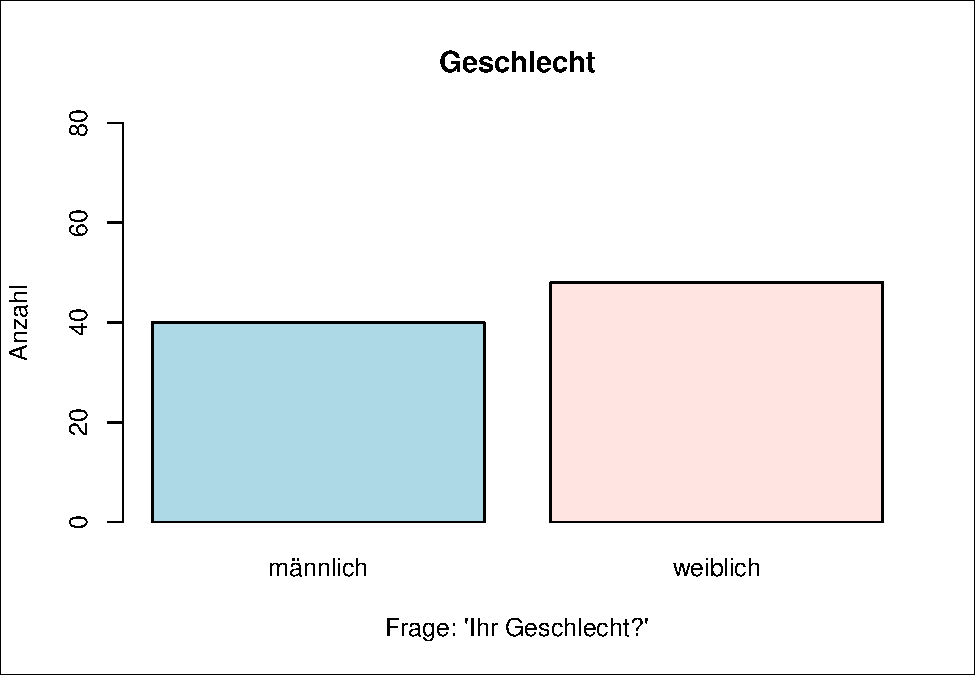
\includegraphics{bericht_files/figure-latex/barplot Geschlecht-1.pdf}

\begin{center}
\textit{Abbildung 1: Frage nach Geschlecht}
\bigskip
\end{center}

\subsection{Prüfung der
Repräsentativität}\label{prufung-der-reprasentativitat}

In Abbildung 1 ist die Verteilung der Befragten nach ihrem Geschlecht
dargestellt. Dabei ist zu erkennen, dass sich unter den Befragten
Personen 53 männliche Studierende und 46 weibliche Studierende befinden.
Dies deutet auf ein Ungleichgewicht hin. Ob die Stichprobe dennoch
repräsentativ ist, kann festgestellt werden, wenn wir die Verteilung
dieser Stichprobe mit der Verteilung der Grundgesamtheit vergleichen.
Die Statistik Austria gibt an, das im Studienjahr 2015/16 insgesamt
21.842 Personen an der WU studiert haben. 11.558 davon sind männliche
und 10.284 sind weibliche Studierende (Statistik Austria, abgerufen am
19.6.2017
\url{https://www.statistik.at/web_de/statistiken/menschen_und_gesellschaft/bildung_und_kultur/formales_bildungswesen/universitaeten_studium/021635.html}).
Wenn wir davon ausgehen, dass sich dieses Verhältnis im Studienjahr
2016/17 nicht verändert hat, ergibt dies eine Verteilung von etwa 53\%
männlichen und 47\% weiblichen Studierenden. Mit einem Chi-Quadrat Test
können wir feststellen, ob sich unsere Stichprobe von der erwarteten
Verteilung der Grundgesamtheit unterscheidet. Die beobachteten und
erwarteten Werte der Verteilung der Geschlechter sehen wir in Tabelle
XY. Für den Chi-Quadrat Test werden folgende Hypothesen aufgestellt:

\begin{longtable}[]{@{}ll@{}}
\toprule
\begin{minipage}[t]{0.11\columnwidth}\raggedright\strut
H\textsubscript{0}:\strut
\end{minipage} & \begin{minipage}[t]{0.83\columnwidth}\raggedright\strut
Die Verteilung der Geschlechter unterscheidet sich nicht von der
erwarteten Verteilung\strut
\end{minipage}\tabularnewline
\begin{minipage}[t]{0.11\columnwidth}\raggedright\strut
H\textsubscript{A}:\strut
\end{minipage} & \begin{minipage}[t]{0.83\columnwidth}\raggedright\strut
Die Verteilung der Geschlechter unterscheidet sich von der erwarteten
Verteilung\strut
\end{minipage}\tabularnewline
\bottomrule
\end{longtable}

Chi-Quadrat Test hierher

\begin{Shaded}
\begin{Highlighting}[]
\CommentTok{#chisq.test(na.omit(fragebogen$sex))}
\KeywordTok{chisq.test}\NormalTok{(}\KeywordTok{c}\NormalTok{(}\FloatTok{10.284}\NormalTok{,}\FloatTok{11.558}\NormalTok{),}\KeywordTok{c}\NormalTok{(sex_count[}\DecValTok{1}\NormalTok{], sex_count[}\DecValTok{2}\NormalTok{]))}
\end{Highlighting}
\end{Shaded}

\begin{verbatim}
## Warning in chisq.test(c(10.284, 11.558), c(sex_count[1], sex_count[2])):
## Chi-squared approximation may be incorrect
\end{verbatim}

\begin{verbatim}
## 
##  Pearson's Chi-squared test with Yates' continuity correction
## 
## data:  c(10.284, 11.558) and c(sex_count[1], sex_count[2])
## X-squared = 0, df = 1, p-value = 1
\end{verbatim}

\subsection{Die abhängige Variable}\label{die-abhangige-variable}

Allen Hypothesen liegt die gleiche abhängige Variable (AV) zugrunde und
lautet: ``Ausmaß der Fremdenfeindlichkeit''. Zur Messung der AV wurde
den Studierenden eine Likertskala mit 10 Items vorgelegt. Die
Antwortmöglichkeiten waren auf einer 6-stufigen Intervallskala mit den
Ausprägungen ``Stimme sehr zu'' bis ``Stimme gar nicht zu'' vorgegeben.
Die Frage lautete ``Wie ist deine Meinung zur Migration?'' (siehe im
Anhang Frage 6 im Fragebogen).

\begin{longtable}[]{@{}ll@{}}
\toprule
\begin{minipage}[b]{0.09\columnwidth}\raggedright\strut
Variablen\strut
\end{minipage} & \begin{minipage}[b]{0.85\columnwidth}\raggedright\strut
Item\strut
\end{minipage}\tabularnewline
\midrule
\endhead
\begin{minipage}[t]{0.09\columnwidth}\raggedright\strut
heimat\strut
\end{minipage} & \begin{minipage}[t]{0.85\columnwidth}\raggedright\strut
Wenn Arbeitsplätze knapp werden, sollte man AusländerInnen wieder in
Ihre Heimat schicken\strut
\end{minipage}\tabularnewline
\begin{minipage}[t]{0.09\columnwidth}\raggedright\strut
rechte\strut
\end{minipage} & \begin{minipage}[t]{0.85\columnwidth}\raggedright\strut
AusländerInnen sollten nicht die gleichen Rechte in allen
Lebensbereichen haben wie ÖsterreicherInnen\strut
\end{minipage}\tabularnewline
\begin{minipage}[t]{0.09\columnwidth}\raggedright\strut
kultur\strut
\end{minipage} & \begin{minipage}[t]{0.85\columnwidth}\raggedright\strut
Ich bin nicht für die Anwesenheit von AusländerInnen weil sie unsere
Kultur negativ beeinflussen\strut
\end{minipage}\tabularnewline
\begin{minipage}[t]{0.09\columnwidth}\raggedright\strut
verlassen\strut
\end{minipage} & \begin{minipage}[t]{0.85\columnwidth}\raggedright\strut
Es wäre am besten, wenn alle AusländerInnen Österreich verlassen
würden\strut
\end{minipage}\tabularnewline
\begin{minipage}[t]{0.09\columnwidth}\raggedright\strut
partner\strut
\end{minipage} & \begin{minipage}[t]{0.85\columnwidth}\raggedright\strut
In Österreich lebende AusländerInnen sollen sich Ihre (Ehe-)partner
unter ihren eigenen Landsleuten wählen\strut
\end{minipage}\tabularnewline
\begin{minipage}[t]{0.09\columnwidth}\raggedright\strut
knapp\strut
\end{minipage} & \begin{minipage}[t]{0.85\columnwidth}\raggedright\strut
Wenn Studierendenplätze an der WU noch knapper werden, sollte man bei
der Zulassung InländerInnen bevorzugen\strut
\end{minipage}\tabularnewline
\begin{minipage}[t]{0.09\columnwidth}\raggedright\strut
pflegen\strut
\end{minipage} & \begin{minipage}[t]{0.85\columnwidth}\raggedright\strut
AusländerInnen sollen ihre Kultur nicht bei uns pflegen, sie sollen sich
an die Kultur in Österreich anpassen\strut
\end{minipage}\tabularnewline
\begin{minipage}[t]{0.09\columnwidth}\raggedright\strut
politik\strut
\end{minipage} & \begin{minipage}[t]{0.85\columnwidth}\raggedright\strut
Politiker sollen sich vor allem für InländerInnen einsetzen\strut
\end{minipage}\tabularnewline
\begin{minipage}[t]{0.09\columnwidth}\raggedright\strut
verdienen\strut
\end{minipage} & \begin{minipage}[t]{0.85\columnwidth}\raggedright\strut
AusländerInnen sollen sich nach dem Zuzug erstmal die Privilegien des
Sozialstaates in Österreich (\ldots{})verdienen\strut
\end{minipage}\tabularnewline
\begin{minipage}[t]{0.09\columnwidth}\raggedright\strut
egal\strut
\end{minipage} & \begin{minipage}[t]{0.85\columnwidth}\raggedright\strut
Wenn ich mit AusländerInnen in einer Arbeitsgruppe bin, ist mir das
nicht egal\strut
\end{minipage}\tabularnewline
\bottomrule
\end{longtable}

Um eine Dimensionsreduktion zu erreichen wird eine
Hauptkomponentenanalyse durchgeführt da die Zuordnung der Items zu
spezifischen Komponenten eine einfachere Interpretation der
Fremdenfeindlichkeit ermöglicht.

NOCH SCHREIBEN: warum item 10 ``egal'' weggelassen (weggelassen weil
Personen vermutlich falsch angekreuzt -\textgreater{} missverständliches
item)

\begin{Shaded}
\begin{Highlighting}[]
\NormalTok{countr <-}\StringTok{ }\KeywordTok{table}\NormalTok{(fragebogen$egal)}
\KeywordTok{rownames}\NormalTok{(countr) <-}\StringTok{ }\KeywordTok{c}\NormalTok{(}\StringTok{"1"}\NormalTok{, }\StringTok{"2"}\NormalTok{, }\StringTok{"3"}\NormalTok{, }\StringTok{"4"}\NormalTok{, }\StringTok{"5"}\NormalTok{, }\StringTok{"6"}\NormalTok{)}
\KeywordTok{barplot}\NormalTok{(countr, }\DataTypeTok{main=}\StringTok{"Variable 'egal'"}\NormalTok{, }\DataTypeTok{ylim=}\KeywordTok{c}\NormalTok{(}\DecValTok{0}\NormalTok{,}\DecValTok{70}\NormalTok{), }\DataTypeTok{xlab=}\StringTok{"Item: 'Wenn ich mit AusländerInnen in einer Arbeitsgruppe bin, ist mir das nicht egal'"}\NormalTok{, }\DataTypeTok{ylab=}\StringTok{"Anzahl"}\NormalTok{)}
\KeywordTok{box}\NormalTok{(}\DataTypeTok{which=}\StringTok{"figure"}\NormalTok{, }\DataTypeTok{lty=}\StringTok{"solid"}\NormalTok{, }\DataTypeTok{col=}\StringTok{"black"}\NormalTok{)}
\end{Highlighting}
\end{Shaded}

\includegraphics{bericht_files/figure-latex/barplot var egal-1.pdf}

Zunächst werden die Voraussetzungen für die Hauptkomponentenanalyse
geprüft.

\begin{Shaded}
\begin{Highlighting}[]
\KeywordTok{library}\NormalTok{(}\StringTok{"psych"}\NormalTok{)}
\CommentTok{# fragebogen[1:2,34:42]}
\NormalTok{av <-}\StringTok{ }\NormalTok{fragebogen[,}\DecValTok{34}\NormalTok{:}\DecValTok{42}\NormalTok{]}
\KeywordTok{nrow}\NormalTok{(av)}
\end{Highlighting}
\end{Shaded}

\begin{verbatim}
## [1] 99
\end{verbatim}

\begin{Shaded}
\begin{Highlighting}[]
\KeywordTok{library}\NormalTok{(}\StringTok{"REdaS"}\NormalTok{)}
\end{Highlighting}
\end{Shaded}

\begin{verbatim}
## Loading required package: grid
\end{verbatim}

\begin{Shaded}
\begin{Highlighting}[]
\KeywordTok{bart_spher}\NormalTok{(av)}
\end{Highlighting}
\end{Shaded}

\begin{verbatim}
##  Bartlett's Test of Sphericity
## 
## Call: bart_spher(x = av)
## 
##      X2 = 486.101
##      df = 36
## p-value < 2.22e-16
\end{verbatim}

Die Teststatistik zeigt ein klares Ergebnis, da die Teststatistik einen
p-Wert unter 0.00000000000000022 erzeugt. Je kleiner der p-Wert ist,
desto mehr Grund gibt es, die Nullhypothese zu verwerfen. Die
Nullhypothese, dass es keine Korrelationen zwischen den Variablen gibt
kann verworfen werden und das Resultat daher als statistisch signifikant
(überzufällig) bezeichnet werden.

\begin{Shaded}
\begin{Highlighting}[]
\NormalTok{kmosmd <-}\StringTok{ }\KeywordTok{KMOS}\NormalTok{(av)}
\KeywordTok{print}\NormalTok{(kmosmd, }\DataTypeTok{stats=}\StringTok{"KMO"}\NormalTok{)}
\end{Highlighting}
\end{Shaded}

\begin{verbatim}
## 
## Kaiser-Meyer-Olkin Statistic
## Call: KMOS(x = av)
## 
## KMO-Criterion: 0.8155905
\end{verbatim}

\begin{Shaded}
\begin{Highlighting}[]
\KeywordTok{print}\NormalTok{(kmosmd, }\DataTypeTok{stats=}\StringTok{"MSA"}\NormalTok{, }\DataTypeTok{sort=}\OtherTok{TRUE}\NormalTok{, }\DataTypeTok{digits=}\DecValTok{3}\NormalTok{, }\DataTypeTok{show=}\DecValTok{1}\NormalTok{:}\DecValTok{5}\NormalTok{)}
\end{Highlighting}
\end{Shaded}

\begin{verbatim}
## 
## Kaiser-Meyer-Olkin Statistics
## 
## Call: KMOS(x = av)
## 
## Measures of Sampling Adequacy (MSA):
## verlassen   pflegen    kultur   partner verdienen 
##     0.709     0.762     0.768     0.795     0.818
\end{verbatim}

Der Wert des KMO liegt bei 0.8155905 und die MSA-Werte liegen bei
\textgreater{} als 0,7. Die Daten sind also als sehr gut geeignet
einzustufen weil genügend Informationen zur Durchführung einer
Hauptkomponentenanalyse vorliegen.

\begin{Shaded}
\begin{Highlighting}[]
\KeywordTok{VSS.scree}\NormalTok{(av)}
\KeywordTok{box}\NormalTok{(}\DataTypeTok{which=}\StringTok{"figure"}\NormalTok{, }\DataTypeTok{lty=}\StringTok{"solid"}\NormalTok{, }\DataTypeTok{col=}\StringTok{"black"}\NormalTok{)}
\end{Highlighting}
\end{Shaded}

\includegraphics{bericht_files/figure-latex/Hauptkomponentenanalyse: Scree plot-1.pdf}

Der Screeplot zeigt, dass die ersten 2 Komponenten einen Eigenwert
\textgreater{} 1 haben, die anderen liegen unter diesem Kriterium.

Komponenten ergeben sich aus der Gruppierung von miteinander
korrelierter Variablen wobei die Komponenten selbst miteinander nicht
korrelieren. Die Gründe des einzelnen Eigenwertes beschreibt den Anteil
der Varianz in den Daten, die durch diese Komponente erklärt wird. Der
Eigenwert wird durch die Anzahl der Items die zu einer Komponente
zusammengefasst werden und der Korrelation innerhalb dieser Gruppe
bestimmt. Je größer der Eigenwert desto mehr trägt er zur Erklärung der
Gesamtstreuung bei. Komponenten mit einem Wert von 1 liefern den
gleichen Erklärungswert wie die einzelne ursprüngliche Variable,
darunter ist der Erklärungswert sogar geringer.

\begin{Shaded}
\begin{Highlighting}[]
\NormalTok{pca.av <-}\StringTok{ }\KeywordTok{principal}\NormalTok{(av, }\DecValTok{2}\NormalTok{, }\DataTypeTok{rotate=}\StringTok{"none"}\NormalTok{)}
\NormalTok{pca.av}
\end{Highlighting}
\end{Shaded}

\begin{verbatim}
## Principal Components Analysis
## Call: principal(r = av, nfactors = 2, rotate = "none")
## Standardized loadings (pattern matrix) based upon correlation matrix
##            PC1   PC2   h2   u2 com
## heimat    0.82  0.28 0.75 0.25 1.2
## rechte    0.62  0.32 0.49 0.51 1.5
## kultur    0.82  0.31 0.77 0.23 1.3
## verlassen 0.67  0.61 0.82 0.18 2.0
## partner   0.59  0.04 0.34 0.66 1.0
## knapp     0.66 -0.43 0.61 0.39 1.7
## pflegen   0.76 -0.42 0.76 0.24 1.6
## politik   0.81 -0.35 0.78 0.22 1.4
## verdienen 0.78 -0.29 0.69 0.31 1.3
## 
##                        PC1  PC2
## SS loadings           4.79 1.23
## Proportion Var        0.53 0.14
## Cumulative Var        0.53 0.67
## Proportion Explained  0.80 0.20
## Cumulative Proportion 0.80 1.00
## 
## Mean item complexity =  1.4
## Test of the hypothesis that 2 components are sufficient.
## 
## The root mean square of the residuals (RMSR) is  0.07 
##  with the empirical chi square  37.83  with prob <  0.0062 
## 
## Fit based upon off diagonal values = 0.98
\end{verbatim}

Komponente PC1 erklärt 53\% der Varianz und Komponente PC2 14\%. Beide
Komponenten zusammen erklären einen Gutteil der Varianz, 67\%, und sind
\textgreater{} 1. Die Hinzunahme weiterer Variablen ist nicht sinnvoll
weil alle weiteren Eigenwerte kleiner als 1 sind.

\begin{Shaded}
\begin{Highlighting}[]
\NormalTok{pca.av_r <-}\StringTok{ }\KeywordTok{principal}\NormalTok{(av, }\DecValTok{2}\NormalTok{)}
\NormalTok{pca.av_r$criteria <-}\StringTok{ }\OtherTok{NULL}
\KeywordTok{print}\NormalTok{(pca.av_r, }\DataTypeTok{cut=}\FloatTok{0.43}\NormalTok{, }\DataTypeTok{sort=}\OtherTok{TRUE}\NormalTok{, }\DataTypeTok{digits=}\DecValTok{3}\NormalTok{)}
\end{Highlighting}
\end{Shaded}

\begin{verbatim}
## Principal Components Analysis
## Call: principal(r = av, nfactors = 2)
## Standardized loadings (pattern matrix) based upon correlation matrix
##           item   RC1   RC2    h2    u2  com
## pflegen      7 0.844       0.761 0.239 1.14
## politik      8 0.829       0.781 0.219 1.27
## knapp        6 0.769       0.612 0.388 1.07
## verdienen    9 0.765       0.690 0.310 1.35
## verlassen    4       0.901 0.816 0.184 1.01
## kultur       3       0.794 0.772 0.228 1.43
## heimat       1       0.769 0.753 0.247 1.51
## rechte       2       0.662 0.489 0.511 1.22
## partner      5       0.431 0.344 0.656 1.99
## 
##                         RC1   RC2
## SS loadings           3.092 2.927
## Proportion Var        0.344 0.325
## Cumulative Var        0.344 0.669
## Proportion Explained  0.514 0.486
## Cumulative Proportion 0.514 1.000
## 
## Mean item complexity =  1.3
## Fit based upon off diagonal values = 0.978
\end{verbatim}

Es werden 2 Hauptkomponenten extrahiert und nach der Varimaxmethode
rotiert. Die Komponenten mit den hoch (\(\ge 0.43\)) auf ihnen ladenden
Variablen sind:

\begin{enumerate}
\def\labelenumi{\arabic{enumi}.}
\tightlist
\item
  Komponente (RC1): moderate Einstellung (Eigenwert: 3.092, erklärte
  Varianz: 34,4\%) ``Bevorzugung von Inländern bei Knappheit von
  Studienplätzen'' .769 ``Anpassung an Kultur in Österreich'' .844
  ``Einsatz Politiker für Inländer'' .829 ``Verdienst Privilegien
  Sozialstaat'' .765
\item
  Komponente (RC2): aggressive Einstellung (Eigenwert: 2.972, erklärte
  Varianz: 32,5\%) ``Wieder in die Heimat schicken'' .769 ``Nicht die
  gleichen Rechte wie Österreicher'' .662 ``Negative Beeinflussung
  Kultur'' .794 ``Österreich verlassen'' .901 ``Ehepartner unter eigenen
  Landsleuten'' .431
\end{enumerate}

\begin{Shaded}
\begin{Highlighting}[]
\KeywordTok{fa.diagram}\NormalTok{(pca.av_r, }\DataTypeTok{cut=}\FloatTok{0.43}\NormalTok{, }\DataTypeTok{cex=}\FloatTok{0.8}\NormalTok{, }\DataTypeTok{rsize=}\FloatTok{0.5}\NormalTok{, }\DataTypeTok{main=}\StringTok{""}\NormalTok{)}
\KeywordTok{box}\NormalTok{(}\DataTypeTok{which=}\StringTok{"figure"}\NormalTok{, }\DataTypeTok{lty=}\StringTok{"solid"}\NormalTok{, }\DataTypeTok{col=}\StringTok{"black"}\NormalTok{)}
\end{Highlighting}
\end{Shaded}

\includegraphics{bericht_files/figure-latex/Hauptkomponentenanalyse: diagramm-1.pdf}

--\textgreater{} Weitere Erklärung noch aus Buch S.465 zb Eine Analyse
der Variablen der 2. Komponente zeigt, dass die gestellten Fragen von
der Mehrheit stark abgelehnt werden -\textgreater{} aggressive
Fragestellung -\textgreater{} hohe Ablehnung -\textgreater{} keine
ausgeprägte Fremdenfeindlichkeit

\begin{Shaded}
\begin{Highlighting}[]
\NormalTok{countr <-}\StringTok{ }\KeywordTok{table}\NormalTok{(fragebogen$rechte)}
\KeywordTok{rownames}\NormalTok{(countr) <-}\StringTok{ }\KeywordTok{c}\NormalTok{(}\StringTok{"1"}\NormalTok{, }\StringTok{"2"}\NormalTok{, }\StringTok{"3"}\NormalTok{, }\StringTok{"4"}\NormalTok{, }\StringTok{"5"}\NormalTok{, }\StringTok{"6"}\NormalTok{)}
\KeywordTok{barplot}\NormalTok{(countr, }\DataTypeTok{main=}\StringTok{"Variable 'rechte'"}\NormalTok{, }\DataTypeTok{ylim=}\KeywordTok{c}\NormalTok{(}\DecValTok{0}\NormalTok{,}\DecValTok{60}\NormalTok{), }\DataTypeTok{xlab=}\StringTok{"Item: AusländerInnen sollten nicht die gleichen Rechte }\CharTok{\textbackslash{}n}\StringTok{ in allen Lebensbereichen haben wie ÖsterreicherInnen"}\NormalTok{, }\DataTypeTok{ylab=}\StringTok{"Anzahl"}\NormalTok{)}
\KeywordTok{box}\NormalTok{(}\DataTypeTok{which=}\StringTok{"figure"}\NormalTok{, }\DataTypeTok{lty=}\StringTok{"solid"}\NormalTok{, }\DataTypeTok{col=}\StringTok{"black"}\NormalTok{)}
\end{Highlighting}
\end{Shaded}

\includegraphics{bericht_files/figure-latex/barplot var rechte-1.pdf}

Für die weitere Analyse werden factor scores angelegt.

\begin{Shaded}
\begin{Highlighting}[]
\KeywordTok{round}\NormalTok{(}\KeywordTok{head}\NormalTok{(pca.av_r$scores), }\DecValTok{4}\NormalTok{)}
\end{Highlighting}
\end{Shaded}

\begin{verbatim}
##       RC1    RC2
## 1  1.3661 0.3307
## 2 -0.4883 0.4607
## 3 -0.0334 0.8614
## 4  1.3661 0.3307
## 5 -0.0516 0.8780
## 6 -0.7460 0.5157
\end{verbatim}

\begin{Shaded}
\begin{Highlighting}[]
\NormalTok{av_r.scores <-}\StringTok{ }\KeywordTok{data.frame}\NormalTok{(pca.av_r$scores)}
\KeywordTok{names}\NormalTok{(av_r.scores) <-}\StringTok{ }\KeywordTok{c}\NormalTok{(}\StringTok{"moderat"}\NormalTok{, }\StringTok{"aggressiv"}\NormalTok{)}
\KeywordTok{round}\NormalTok{(}\KeywordTok{head}\NormalTok{(av_r.scores), }\DecValTok{4}\NormalTok{)}
\end{Highlighting}
\end{Shaded}

\begin{verbatim}
##   moderat aggressiv
## 1  1.3661    0.3307
## 2 -0.4883    0.4607
## 3 -0.0334    0.8614
## 4  1.3661    0.3307
## 5 -0.0516    0.8780
## 6 -0.7460    0.5157
\end{verbatim}

\begin{Shaded}
\begin{Highlighting}[]
\CommentTok{# Weitere Analyse mit den folgenden beiden Variablen:}
\NormalTok{av_r.scores$moderat}
\end{Highlighting}
\end{Shaded}

\begin{verbatim}
##  [1]  1.366091e+00 -4.883442e-01 -3.339595e-02  1.366091e+00 -5.157928e-02
##  [6] -7.460068e-01 -2.228172e+00  1.885807e-01 -1.008100e+00  5.181124e-01
## [11] -1.461072e+00 -1.520975e+00  1.188650e+00  2.527261e-01 -8.804113e-02
## [16] -8.017079e-01 -5.275213e-01 -6.425426e-01  1.366091e+00  1.366091e+00
## [21] -8.773640e-01 -1.707386e+00 -8.064045e-01 -4.932594e-01 -4.262787e-01
## [26] -7.329794e-01 -2.149755e+00 -2.477882e-01  1.366091e+00 -3.247262e-01
## [31]  9.648289e-01  1.366091e+00  6.000234e-01  7.019214e-01  1.629138e+00
## [36]  1.366091e+00 -2.608005e-01 -1.566282e-01  5.916297e-02  2.177391e+00
## [41] -6.043733e-01 -5.086249e-01 -1.320391e-01 -1.088600e+00  1.629138e+00
## [46]  1.169882e+00  7.762045e-01 -2.210222e+00  2.003489e-01 -1.401177e-01
## [51]  6.350812e-01  4.343351e-01  2.402967e-01 -2.302441e-01  2.175294e-01
## [56]  8.495617e-01  1.366091e+00  1.366091e+00  1.366091e+00 -8.488815e-01
## [61] -1.211061e+00  1.188650e+00  2.568942e-01 -2.111124e+00 -1.147838e+00
## [66] -2.864318e-02 -2.613852e-01 -1.525991e+00 -8.730946e-01  6.423122e-01
## [71] -3.281128e-02 -1.267839e+00  7.462686e-01 -1.442374e+00 -4.492347e-01
## [76]  7.451459e-02 -4.122141e-01 -3.675397e-01  1.366091e+00  1.366091e+00
## [81] -3.746807e-01  4.854804e-05  1.128492e-01  8.785518e-01 -2.628421e-01
## [86] -4.582365e-02  3.408385e-01 -1.524328e+00  9.924412e-01 -8.757256e-01
## [91] -1.433988e+00  2.772772e-01  5.682431e-01 -4.557166e-01 -5.476288e-01
## [96]  6.740465e-01  6.450049e-01  6.057791e-01  1.366091e+00
\end{verbatim}

\begin{Shaded}
\begin{Highlighting}[]
\NormalTok{av_r.scores$aggressiv}
\end{Highlighting}
\end{Shaded}

\begin{verbatim}
##  [1]  0.33074730  0.46072646  0.86139672  0.33074730  0.87796460
##  [6]  0.51574894  1.42449083  0.49569675  1.17489060 -0.35964818
## [11] -0.66561700 -0.62774722  0.36935596  0.46236938  0.29041014
## [16]  0.20975880  0.30366879  0.14544555  0.33074730  0.33074730
## [21]  0.10299877  1.17681145 -1.94544408  0.36372050 -1.94928602
## [26]  0.99615210  0.49923009  0.96919665  0.33074730  0.81426257
## [31]  0.31182106  0.33074730  0.64305211 -0.03267838 -0.49515657
## [36]  0.33074730  0.91520918 -0.45616121  0.40362445 -3.66540232
## [41] -0.38956631 -1.12840965 -2.29879784  1.07349664 -0.49515657
## [46]  0.42197935  0.14515305 -0.55336772  0.66491789 -1.10283752
## [51] -0.09298379  0.27635784 -2.07030825 -2.54519127  0.57150248
## [56] -2.96047074  0.33074730  0.33074730  0.33074730 -1.80650166
## [61]  0.66677411  0.36935596  0.31496650 -0.35662517  0.95929390
## [66]  0.67793833  0.95126470  0.52562738 -2.59727227  0.35434694
## [71]  0.82534121  0.10800217  0.56702386  0.24810343 -0.62273664
## [76]  0.46149824  0.05946390 -0.27804394  0.33074730  0.33074730
## [81]  0.95654599  0.37130120  0.78536847  0.37484520 -1.26289106
## [86]  0.77135374  0.69550050  0.52329675  0.46058801 -1.56024683
## [91] -2.81945581 -0.47272624  0.64168804 -0.03068128  0.26608368
## [96]  0.27527097 -0.34699752  0.53644126  0.33074730
\end{verbatim}

In der weiteren Analyse wird mit zwei metrischen Variablen
weitergearbeitet.

\subsection{Hypothese 1}\label{hypothese-1}

\subsection{Hypothese 2}\label{hypothese-2}

\subsection{Hypothese 3}\label{hypothese-3}

\subsubsection{Problemanalyse}\label{problemanalyse}

In diesem Abschnitt wollen wir überprüfen, ob die Einstellung der
Studierenden abhängig von der Einstellung der Personen in Ihrem sozialen
Umfeld ist.

Unsere Hypothese dazu latüt: \emph{Je mehr Menschen im persönlichen
Umfeld (Freunde, Familie) ausländerfeindlich sind, umso negativer ist
die eigene Haltung gegenüber AusländerInnen.}

\paragraph{Welche Variablen kommen
vor?}\label{welche-variablen-kommen-vor}

Erklärende Variable: Umfeld

Besteht aus neun Items; --\textgreater{} metrisch

Responsevariable: Fremdenfeindlichkeit

Wurde bereits im Kapitel x behandelt; Die Ergebnisse werden für die
Analyse weiterverwendet

\begin{itemize}
\item
  av\_r.scores\$moderat, Fremdenfeindlichkeit ``moderat''``, metrisch
\item
  av\_r.scores\$aggressiv, Fremdenfeindlichkeit ``aggressiv'', metrisch
\end{itemize}

\paragraph{Welche Methode ist
angebracht?}\label{welche-methode-ist-angebracht}

t-Test

\paragraph{Welche Hypothesen können formuliert
werden?}\label{welche-hypothesen-konnen-formuliert-werden}

\begin{longtable}[]{@{}ll@{}}
\toprule
\begin{minipage}[t]{0.13\columnwidth}\raggedright\strut
H\textsubscript{0}:\strut
\end{minipage} & \begin{minipage}[t]{0.81\columnwidth}\raggedright\strut
~~Die eigene Einstellung zu MigratenInnen ist unabhängig von der
Einstellung der Personen im eigenen Umfeld.\strut
\end{minipage}\tabularnewline
\begin{minipage}[t]{0.13\columnwidth}\raggedright\strut
H\textsubscript{A}:\strut
\end{minipage} & \begin{minipage}[t]{0.81\columnwidth}\raggedright\strut
~~Die eigene Einstellung zu MigratenInnen ist abhängig von der
Einstellung der Personen im eigenen Umfeld.\strut
\end{minipage}\tabularnewline
\bottomrule
\end{longtable}

\paragraph{Die unabhängige Variable -
Umfeld}\label{die-unabhangige-variable---umfeld}

\begin{longtable}[]{@{}ll@{}}
\toprule
\begin{minipage}[b]{0.09\columnwidth}\raggedright\strut
Variablen\strut
\end{minipage} & \begin{minipage}[b]{0.85\columnwidth}\raggedright\strut
Item\strut
\end{minipage}\tabularnewline
\midrule
\endhead
\begin{minipage}[t]{0.09\columnwidth}\raggedright\strut
diskut\strut
\end{minipage} & \begin{minipage}[t]{0.85\columnwidth}\raggedright\strut
Ich diskutiere mit meinen Familienmitgliedern/Freunden oft über
AusländerInnen\strut
\end{minipage}\tabularnewline
\begin{minipage}[t]{0.09\columnwidth}\raggedright\strut
scherzen\strut
\end{minipage} & \begin{minipage}[t]{0.85\columnwidth}\raggedright\strut
Ich kenne Familienmitglieder/Freunde, die oft über AusländerInnen im
negativen Sinne scherzen\strut
\end{minipage}\tabularnewline
\begin{minipage}[t]{0.09\columnwidth}\raggedright\strut
erfahrung\strut
\end{minipage} & \begin{minipage}[t]{0.85\columnwidth}\raggedright\strut
Einige meiner Familienmitglieder/Freunde haben bereits negative
Erfahrungen mit AusländerInnen gemacht\strut
\end{minipage}\tabularnewline
\begin{minipage}[t]{0.09\columnwidth}\raggedright\strut
demo\strut
\end{minipage} & \begin{minipage}[t]{0.85\columnwidth}\raggedright\strut
Ich würde einigen meiner Familienmitglieder/Freunde zutraün, dass Sie
bei Demonstrationen gegen AusländerInnen teilnehmen\strut
\end{minipage}\tabularnewline
\begin{minipage}[t]{0.09\columnwidth}\raggedright\strut
gewalt\strut
\end{minipage} & \begin{minipage}[t]{0.85\columnwidth}\raggedright\strut
Heutzutage muss man Verständnis haben, wenn Familienmitglieder/Freunde
Gewalt gegen AusländerInnen ausüben müssen\strut
\end{minipage}\tabularnewline
\begin{minipage}[t]{0.09\columnwidth}\raggedright\strut
krimi\strut
\end{minipage} & \begin{minipage}[t]{0.85\columnwidth}\raggedright\strut
Ich kenne Familienmitglieder/Freunde, die AusländerInnen für Kriminelle
halten\strut
\end{minipage}\tabularnewline
\begin{minipage}[t]{0.09\columnwidth}\raggedright\strut
fpö \textbar{}\strut
\end{minipage} & \begin{minipage}[t]{0.85\columnwidth}\raggedright\strut
Ich kenne Familienmitglieder/Freunde, die FPÖ wählen\strut
\end{minipage}\tabularnewline
\begin{minipage}[t]{0.09\columnwidth}\raggedright\strut
sicherheit\strut
\end{minipage} & \begin{minipage}[t]{0.85\columnwidth}\raggedright\strut
Seit der Flüchtlingskrise haben einige meiner Familienmitglieder/Freunde
Angst um Ihre eigene Sicherheit\strut
\end{minipage}\tabularnewline
\begin{minipage}[t]{0.09\columnwidth}\raggedright\strut
feindlich\strut
\end{minipage} & \begin{minipage}[t]{0.85\columnwidth}\raggedright\strut
Ich kenne Familienmitglieder/Freunde,die fremdenfeindlich sind\strut
\end{minipage}\tabularnewline
\bottomrule
\end{longtable}

\begin{center}
\textit{Tabelle 2: Unabhängige Variable: Umfeld}
\bigskip
\end{center}

\subsubsection{Kurzbericht}\label{kurzbericht}

Die Einstellung der Personen im sozialen Umfeld wurde anhand von neun
Items überprüft. Die übergerordente Frage dazu lautet: ``Einstellung zur
Migration in deinem sozialen Umfeld?'' Als Maßstab wurde eine
Intervallskala von eins bis sechs verwendet, wobei 1 = ``Trifft sehr
zu'' und 6 = ``Trifft gar nicht zu''.

Da wir hier mit multivairate Datean zu tun haben, wird eine
Hauptkomponentenanalyse durchtgeführt, um die Datendimension zu
reduzieren.

\paragraph{Voraussetzungen für die
Hauptkomponentenanalyse}\label{voraussetzungen-fur-die-hauptkomponentenanalyse}

Bevor wir die Voraussetzungen überprüfen, müssen wir die richtigen Daten
auswählen. Wir werden alle Daten mit NAs entfernen und schaün uns das
Ergebniss an.

\begin{Shaded}
\begin{Highlighting}[]
\KeywordTok{library}\NormalTok{(}\StringTok{"psych"}\NormalTok{)}
\KeywordTok{library}\NormalTok{(}\StringTok{"zoo"}\NormalTok{)}
\end{Highlighting}
\end{Shaded}

\begin{verbatim}
## 
## Attaching package: 'zoo'
\end{verbatim}

\begin{verbatim}
## The following objects are masked from 'package:base':
## 
##     as.Date, as.Date.numeric
\end{verbatim}

\begin{Shaded}
\begin{Highlighting}[]
\NormalTok{umfeld<-}\KeywordTok{na.omit}\NormalTok{((fragebogen[,}\DecValTok{19}\NormalTok{:}\DecValTok{27}\NormalTok{]))}
\KeywordTok{nrow}\NormalTok{(umfeld)}
\end{Highlighting}
\end{Shaded}

\begin{verbatim}
## [1] 94
\end{verbatim}

Wenn wir für die ausgewählten Items alle Zeilen wo mindestens ein NA
vorkommt entfernen, dann bleiben uns in Summe nur noch 94 Datensätze
übrig. An erster Stelle ist es natürlich Schade, Datensätze wegen ein
bis zwei NA zu entfernen. Aber wir erinnern uns zurück, dass wir für die
abhängige Variable ``Fremdenfeindlichkeit'' 99 Datensätze verwendet
haben.

Damit wir gleich vielen Daten für die abhängige- und unabhängige
Variable verwenden können, werden wir die Rohdaten wieder hernehmen und
fehlende Einträge mit der \emph{na.approx}-Funktion ergänzen. Und danach
die Datensätze mit der ``!is.na''-Funktion auf jene Daten reduziert, die
in der Variable ``Heimat'', welche im Datensatz der
Hautpkomponentenanalyse der ``Fremdenfeindlichkeit'' vorkommt.

\begin{Shaded}
\begin{Highlighting}[]
\KeywordTok{library}\NormalTok{(}\StringTok{"psych"}\NormalTok{)}
\KeywordTok{library}\NormalTok{(}\StringTok{"zoo"}\NormalTok{)}
\NormalTok{umfeld<-}\KeywordTok{na.approx}\NormalTok{(fragebogen[,}\DecValTok{19}\NormalTok{:}\DecValTok{27}\NormalTok{])}
\NormalTok{umfeld<-umfeld[!}\KeywordTok{is.na}\NormalTok{(av[}\StringTok{"heimat"}\NormalTok{]),]}
\KeywordTok{nrow}\NormalTok{(umfeld)}
\end{Highlighting}
\end{Shaded}

\begin{verbatim}
## [1] 99
\end{verbatim}

Jetzt haben wir exakt 99 Datensätze, die mit der abhängigen Varialbe
``Fremdenfeindlichkeit'' übereintimmen.

\subparagraph{\texorpdfstring{Bartlett-Test:
``Umfeld''}{Bartlett-Test: Umfeld}}\label{bartlett-test-umfeld}

Nachdem unser Datensatz für die weitere Bearbeitung dementsprechend
vorbereitet wuden, können wir nun mit der überprüfung der
Voraussetzungen für die Hauptkomponentenanalyse loslegen.

Als Erstes führen wir den Bartlett-Test durch:

\begin{Shaded}
\begin{Highlighting}[]
\KeywordTok{library}\NormalTok{(}\StringTok{"REdaS"}\NormalTok{)}
\KeywordTok{bart_spher}\NormalTok{(umfeld)}
\end{Highlighting}
\end{Shaded}

\begin{verbatim}
##  Bartlett's Test of Sphericity
## 
## Call: bart_spher(x = umfeld)
## 
##      X2 = 312.309
##      df = 36
## p-value < 2.22e-16
\end{verbatim}

Die Teststatistik zeigt ein klares Ergebnis, da die Teststatistik
\(X^2=312.309\) mit einer \(\chi^2\)-Verteilung mit 36 Freiheitsgraden
einen p-Wert unter 0.00000000000000022 erzeugt. Je kleiner der p-Wert
ist, desto mehr Grund gibt es, die Nullhypothese zu verwerfen. Die
Nullhypothese, dass es keine Korrelationen zwischen den Variablen gibt
kann verworfen werden und das Resultat daher als statistisch signifikant
bezeichnet werden.

\subparagraph{\texorpdfstring{KMO und MSA:
``Umfeld''}{KMO und MSA: Umfeld}}\label{kmo-und-msa-umfeld}

Als nüchstes werden wir die MSAs und die KMO überprüfen.

\begin{Shaded}
\begin{Highlighting}[]
\NormalTok{kmosmd <-}\StringTok{ }\KeywordTok{KMOS}\NormalTok{(umfeld)}
\KeywordTok{print}\NormalTok{(kmosmd, }\DataTypeTok{stats=}\StringTok{"KMO"}\NormalTok{)}
\end{Highlighting}
\end{Shaded}

\begin{verbatim}
## 
## Kaiser-Meyer-Olkin Statistic
## Call: KMOS(x = umfeld)
## 
## KMO-Criterion: 0.8040357
\end{verbatim}

\begin{Shaded}
\begin{Highlighting}[]
\KeywordTok{print}\NormalTok{(kmosmd, }\DataTypeTok{stats=}\StringTok{"MSA"}\NormalTok{, }\DataTypeTok{sort=}\OtherTok{TRUE}\NormalTok{, }\DataTypeTok{digits=}\DecValTok{3}\NormalTok{, }\DataTypeTok{show=}\DecValTok{1}\NormalTok{:}\DecValTok{5}\NormalTok{)}
\end{Highlighting}
\end{Shaded}

\begin{verbatim}
## 
## Kaiser-Meyer-Olkin Statistics
## 
## Call: KMOS(x = umfeld)
## 
## Measures of Sampling Adequacy (MSA):
##     gewalt sicherheit  erfahrung     diskut       demo 
##      0.626      0.687      0.769      0.816      0.828
\end{verbatim}

Der Wert des KMO liegt bei 0.8040357 und die MSA-Werte liegen bei
\textgreater{} als 0,6. Die Daten sind also als sehr gut geeignet
einzustufen weil genügend Informationen zur Durchführung einer
Hauptkomponentenanalyse vorliegen.

\subparagraph{Scree Plot: Umfeld}\label{scree-plot-umfeld}

Mittels Scree Plot können wir nun überprüfen, wieviele Hauptkomponenten
für die Hauptkomponentennalyse benötigt werden.

\begin{Shaded}
\begin{Highlighting}[]
\KeywordTok{VSS.scree}\NormalTok{(umfeld)}
\KeywordTok{box}\NormalTok{(}\DataTypeTok{which=}\StringTok{"figure"}\NormalTok{, }\DataTypeTok{lty=}\StringTok{"solid"}\NormalTok{, }\DataTypeTok{col=}\StringTok{"black"}\NormalTok{)}
\end{Highlighting}
\end{Shaded}

\includegraphics{bericht_files/figure-latex/Umfeld: Scree plot-1.pdf}

\begin{center}
\textit{Abbildung 2: Scree Plot:Umfeld}
\bigskip
\end{center}

Der Screeplot zeigt, dass die ersten 2 Komponenten einen Eigenwert
\textgreater{} 1 haben, die anderen liegen unter diesem Kriterium.

\subparagraph{\texorpdfstring{Hauptkomponentenanalyse:
``Umfeld''}{Hauptkomponentenanalyse: Umfeld}}\label{hauptkomponentenanalyse-umfeld}

Basierend auf der Information aus dem Screeplot werden wir im ersten
Versuch zwei Komponenten extrahieren und vorerst keine Rotation
durchführen. Um den Output zu reduzieren, wird die Objektkomponente
\emph{criteria} entfernt.

\begin{Shaded}
\begin{Highlighting}[]
\NormalTok{pca.umfeld <-}\StringTok{ }\KeywordTok{principal}\NormalTok{(umfeld, }\DecValTok{2}\NormalTok{, }\DataTypeTok{rotate=}\StringTok{"none"}\NormalTok{)}
\NormalTok{pca.umfeld$criteria<-}\OtherTok{NULL}
\NormalTok{pca.umfeld}
\end{Highlighting}
\end{Shaded}

\begin{verbatim}
## Principal Components Analysis
## Call: principal(r = umfeld, nfactors = 2, rotate = "none")
## Standardized loadings (pattern matrix) based upon correlation matrix
##             PC1   PC2   h2   u2 com
## diskut     0.46  0.23 0.27 0.73 1.5
## scherzen   0.71  0.12 0.51 0.49 1.1
## erfahrung  0.69 -0.26 0.55 0.45 1.3
## demo       0.72  0.25 0.58 0.42 1.2
## gewalt     0.44  0.68 0.65 0.35 1.7
## krimi      0.78  0.17 0.64 0.36 1.1
## fpoe       0.72 -0.13 0.53 0.47 1.1
## sicherheit 0.58 -0.61 0.70 0.30 2.0
## feindlich  0.82 -0.21 0.72 0.28 1.1
## 
##                        PC1  PC2
## SS loadings           4.04 1.12
## Proportion Var        0.45 0.12
## Cumulative Var        0.45 0.57
## Proportion Explained  0.78 0.22
## Cumulative Proportion 0.78 1.00
## 
## Mean item complexity =  1.3
## Fit based upon off diagonal values = 0.94
\end{verbatim}

Komponente PC1 erklärt 45\% der Varianz und Komponente PC2 12\%. Beide
Komponenten zusammen erklären 57\% und sind \textgreater{} 1. Die
Hinzunahme weiterer Variablen ist nicht sinnvoll weil alle weiteren
Eigenwerte kleiner als 1 sind.

\subparagraph{Varimax-Rotation: Umfeld}\label{varimax-rotation-umfeld}

Es werden zwei Hauptkomponenten extrahiert und nach der Varimaxmethode
rotiert.

\begin{Shaded}
\begin{Highlighting}[]
\NormalTok{pca.umfeld_r <-}\StringTok{ }\KeywordTok{principal}\NormalTok{(umfeld, }\DecValTok{2}\NormalTok{)}
\NormalTok{pca.umfeld_r$criteria <-}\StringTok{ }\OtherTok{NULL}
\KeywordTok{print}\NormalTok{(pca.umfeld_r, }\DataTypeTok{cut=}\FloatTok{0.48}\NormalTok{, }\DataTypeTok{sort=}\OtherTok{TRUE}\NormalTok{, }\DataTypeTok{digits=}\DecValTok{3}\NormalTok{)}
\end{Highlighting}
\end{Shaded}

\begin{verbatim}
## Principal Components Analysis
## Call: principal(r = umfeld, nfactors = 2)
## Standardized loadings (pattern matrix) based upon correlation matrix
##            item    RC1    RC2    h2    u2  com
## sicherheit    8  0.834        0.701 0.299 1.02
## feindlich     9  0.756        0.720 0.280 1.49
## erfahrung     3  0.694        0.549 0.451 1.27
## fpoe          7  0.624        0.530 0.470 1.64
## gewalt        5         0.800 0.654 0.346 1.04
## demo          4         0.664 0.583 0.417 1.59
## krimi         6         0.642 0.640 0.360 1.85
## scherzen      2         0.558 0.513 0.487 1.91
## diskut        1         0.481 0.268 0.732 1.32
## 
##                         RC1   RC2
## SS loadings           2.761 2.396
## Proportion Var        0.307 0.266
## Cumulative Var        0.307 0.573
## Proportion Explained  0.535 0.465
## Cumulative Proportion 0.535 1.000
## 
## Mean item complexity =  1.5
## Fit based upon off diagonal values = 0.939
\end{verbatim}

Es werden zwei Hauptkomponenten extrahiert und nach der Varimaxmethode
rotiert. Die Komponenten mit den hoch (\(\ge 0.48\)) auf ihnen ladenden
Variablen sind:

\begin{enumerate}
\def\labelenumi{\arabic{enumi}.}
\tightlist
\item
  Komponente (RC1): Passives Umfeld (Eigenwert: 2.761, erklärte Varianz:
  30,7\%) ``Angst um die eigene Sicherheit'' .834 ``Fremdenfeindliche
  Personen im Umfeld'' .756 ``Bereits negative Erfahrung mit
  AusländerInnen'' .694 ``FPÖ-Wähler im Umfeld'' .624
\item
  Komponente (RC2): Aktives Umfeld (Eigenwert: 2.396, erklärte Varianz:
  26,6\%) ``Gewalt ausüben'' .8 ``Bei Demosnstrationen gegen
  AusländerInnen teilnehmen'' .664 ``AuländerInnen für Kriminelle
  halten'' .642 ``über AusländerInnen scherzen'' .558 ``über
  AusländerInnen diskutieren'' .481
\end{enumerate}

\subparagraph{\texorpdfstring{Zuordnung der Items:
``Umfeld''}{Zuordnung der Items: Umfeld}}\label{zuordnung-der-items-umfeld}

Als nüchstes schaün wir uns die Ergebnisse grafisch an.

\begin{Shaded}
\begin{Highlighting}[]
\KeywordTok{fa.diagram}\NormalTok{(pca.umfeld_r, }\DataTypeTok{cut=}\FloatTok{0.43}\NormalTok{, }\DataTypeTok{cex=}\FloatTok{0.8}\NormalTok{, }\DataTypeTok{rsize=}\FloatTok{0.5}\NormalTok{, }\DataTypeTok{main=}\StringTok{""}\NormalTok{)}
\KeywordTok{box}\NormalTok{(}\DataTypeTok{which=}\StringTok{"figure"}\NormalTok{, }\DataTypeTok{lty=}\StringTok{"solid"}\NormalTok{, }\DataTypeTok{col=}\StringTok{"black"}\NormalTok{)}
\end{Highlighting}
\end{Shaded}

\includegraphics{bericht_files/figure-latex/Umfeld PCA: diagram-1.pdf}

\begin{center}
\textit{Abbildung 3: Fa-Diagram: Umfeld}
\bigskip
\end{center}

Anhand der durchwegs positiven Ladungen kann man erkennen, dass Personen
mit hohen Werten bei den jeweiligen Items auch hohe Auspr?gungen auf der
Komponente haben. Die zwei extrahierten Hauptkomponenten sind direkt
interpretierbar als ``aktives-'' und ``passives Umfeld''. Menschen die
bereit sind Gewalt gegen AusländerInnen auszuüben, bei Demonstrationen
teilzunehmen, über Ausländer scherzen und diskutieren oder diese für
Kriminelle halten, befinden sich auf der aktiven Seiten.

\subparagraph{\texorpdfstring{Factor Scores:
``Umfeld''}{Factor Scores: Umfeld}}\label{factor-scores-umfeld}

für die weitere Analyse werden factor scores angelegt.

\begin{Shaded}
\begin{Highlighting}[]
\KeywordTok{round}\NormalTok{(}\KeywordTok{head}\NormalTok{(pca.umfeld_r$scores), }\DecValTok{4}\NormalTok{)}
\end{Highlighting}
\end{Shaded}

\begin{verbatim}
##          RC1     RC2
## [1,] -0.7416 -0.0137
## [2,] -0.3407  0.8159
## [3,]  1.0228  0.7525
## [4,]  1.3662  0.1100
## [5,] -0.9171 -0.1063
## [6,]  0.5026  0.7708
\end{verbatim}

\begin{Shaded}
\begin{Highlighting}[]
\NormalTok{umfeld_r.scores <-}\StringTok{ }\KeywordTok{data.frame}\NormalTok{(pca.umfeld_r$scores)}
\KeywordTok{names}\NormalTok{(umfeld_r.scores) <-}\StringTok{ }\KeywordTok{c}\NormalTok{(}\StringTok{"passiv"}\NormalTok{, }\StringTok{"aktiv"}\NormalTok{)}
\KeywordTok{round}\NormalTok{(}\KeywordTok{head}\NormalTok{(umfeld_r.scores), }\DecValTok{4}\NormalTok{)}
\end{Highlighting}
\end{Shaded}

\begin{verbatim}
##    passiv   aktiv
## 1 -0.7416 -0.0137
## 2 -0.3407  0.8159
## 3  1.0228  0.7525
## 4  1.3662  0.1100
## 5 -0.9171 -0.1063
## 6  0.5026  0.7708
\end{verbatim}

\begin{Shaded}
\begin{Highlighting}[]
\CommentTok{# Weitere Analyse mit den folgenden beiden Variablen:}
\NormalTok{umfeld_r.scores$passiv}
\end{Highlighting}
\end{Shaded}

\begin{verbatim}
##  [1] -0.74162049 -0.34069773  1.02277703  1.36624408 -0.91709156
##  [6]  0.50257924 -0.28787047  1.39297226 -0.29674112  1.20436535
## [11] -0.08211912 -0.58425545  1.39959899  0.31154646 -0.07274143
## [16] -0.59687912 -0.53761796 -1.02250005  1.48654333  0.24074306
## [21]  0.69104841  0.26148127  0.01732844  0.26785772 -0.29189852
## [26]  0.51504005 -1.05209634  1.33903607  0.42980979 -0.21143500
## [31] -0.18695940  0.52391305 -0.10047140 -1.53108045 -1.29568541
## [36]  0.51309767 -0.19503007  0.61385698  0.54001928  1.05322026
## [41] -0.47019345 -1.52633469 -0.11409551 -1.85814944 -0.37397494
## [46] -0.52915935 -0.05775366 -0.67506252  0.85433033  0.04113291
## [51] -1.85301447 -0.42397250 -1.01297461  1.52572883  1.48216314
## [56]  0.72574588  1.60145424 -0.12040041  1.16982914  0.07726273
## [61] -0.77918691  1.56096381 -1.74612719 -0.18119992 -0.45956690
## [66]  0.22015353  1.62315118 -0.04728601 -0.88615866 -1.46385148
## [71] -0.15619856 -0.94795952  0.60956393  0.94679048 -1.96465345
## [76]  0.99737002 -0.68416797  2.15643833  1.63747710  0.33969053
## [81] -0.74732787 -1.16111061  1.56691802  1.10006025  0.31142305
## [86] -1.11541827  0.56894319 -0.51021129  0.75939892 -0.60809049
## [91] -2.15014303 -1.03124291  1.40174060 -2.03131571 -1.54329830
## [96]  0.82890372 -0.64390921 -0.46291524  0.88150351
\end{verbatim}

\begin{Shaded}
\begin{Highlighting}[]
\NormalTok{umfeld_r.scores$aktiv}
\end{Highlighting}
\end{Shaded}

\begin{verbatim}
##  [1] -0.013719474  0.815949448  0.752477658  0.109965840 -0.106272527
##  [6]  0.770817455 -0.255141911  0.423550502 -0.544030411  0.623260277
## [11]  1.089432843 -0.250822318  1.030692653  0.906416750  0.478739774
## [16]  0.136978499  0.273225630  0.795618033 -0.418002634  0.615734420
## [21] -0.490530154  0.675567958 -3.315231116  0.507448521 -0.636525182
## [26]  1.139288453  1.411228461 -1.731832633 -0.003400310  0.615862248
## [31]  1.188783793 -3.874778150 -1.674300560 -0.626290887  0.968380839
## [36]  0.197708629 -0.006406447  0.776843715  0.843716126 -1.615809458
## [41] -1.077824674 -0.713034999  0.329078769  0.022077310  1.429851199
## [46]  0.488374111  0.994330502 -1.954319670  0.183607813 -1.787679645
## [51] -0.308586976 -0.120512178  0.148184104 -2.436312372  0.135106425
## [56]  0.540328399  0.832007236 -0.187398030  0.509045471 -0.883588429
## [61] -1.240604638 -0.564841839  0.014208927  0.043417340 -0.469657871
## [66]  0.690054024  0.207439036 -1.255395060 -2.927407266  0.483173260
## [71] -0.159163829  0.344814633  0.692355860 -0.190130196  0.037640319
## [76] -0.060649964  0.483770501 -0.656813571  0.670768534  1.433102990
## [81]  0.075945222  0.796870801  0.717792429  0.911338417 -0.678710889
## [86]  0.182276354  0.455125153 -0.249794288  0.953859122 -1.249966564
## [91] -0.119478738  0.785869509  0.063628652  0.117673182  1.021930656
## [96]  0.136343902 -0.510870570  1.631509667 -0.344751928
\end{verbatim}

\paragraph{überprüfung der Hypothesen}\label{uberprufung-der-hypothesen}

In der weiteren Analyse wird mit vier metrischen Variablen
weitergearbeitet.

Responsevariable ``Fremdenfeindlichkeit'': Moderat und Aggressiv

Erklärende Variable ``Umfeld'': Aktiv und Passiv

Mittels linearen Regressionsmodells sollen die Responsevariablen durch
die erklärende Variablen beschreiben werden. Ein Streudiagramm ist eine
geeignete Variante, um den Zusammenhang bildhaft überprüfen zu können.

\subparagraph{Moderat und Passiv}\label{moderat-und-passiv}

In diesem Streudiagramm ist die Responsebariable (Moderat) auf der
y-Achse und die erklärende Variable (Passiv) auf der x-Achse. Anhand der
\emph{lm()}-Funktion erfolgt die Schätzung des Modells. Die Schätzung
kann für zwei Zwecke verwendet werden. Als erstes benötigen wir sie, um
eine Gerade im Streudiagrmam mit der Funkton \emph{abline()} einzeichnen
zu können. Und später können wir die Ergebnisse für den \emph{t-test für
den Regressionsköffizienten} verwenden.

\begin{Shaded}
\begin{Highlighting}[]
\NormalTok{mopa<-}\KeywordTok{lm}\NormalTok{(av_r.scores$moderat ~}\StringTok{ }\NormalTok{umfeld_r.scores$passiv)}
\KeywordTok{plot}\NormalTok{(umfeld_r.scores$passiv, av_r.scores$moderat, }\DataTypeTok{xlab=}\StringTok{"Passiv"}\NormalTok{, }\DataTypeTok{ylab=}\StringTok{"Moderat"}\NormalTok{)}
\KeywordTok{abline}\NormalTok{(mopa)}
\end{Highlighting}
\end{Shaded}

\includegraphics{bericht_files/figure-latex/boxplot: moderat - Passiv-1.pdf}

\begin{center}
\textit{Abbildung 4: Boxplot: Moderat und Passiv}
\bigskip
\end{center}

Nachdem das Steudiagramm nicht eindeutig ist, führen wir im nüchsten
Schritt einen \emph{t-test} durch.

\subparagraph{T-test: Moderat und
Passiv}\label{t-test-moderat-und-passiv}

Die Schätzung haben wir bereits ausgerechnent, und können mit
\emph{summary()} ausgeben.

\begin{Shaded}
\begin{Highlighting}[]
\KeywordTok{summary}\NormalTok{(mopa)}
\end{Highlighting}
\end{Shaded}

\begin{verbatim}
## 
## Call:
## lm(formula = av_r.scores$moderat ~ umfeld_r.scores$passiv)
## 
## Residuals:
##      Min       1Q   Median       3Q      Max 
## -2.13209 -0.63763 -0.08479  0.74963  2.06159 
## 
## Coefficients:
##                         Estimate Std. Error t value Pr(>|t|)    
## (Intercept)            2.907e-17  9.523e-02   0.000 1.000000    
## umfeld_r.scores$passiv 3.338e-01  9.571e-02   3.487 0.000735 ***
## ---
## Signif. codes:  0 '***' 0.001 '**' 0.01 '*' 0.05 '.' 0.1 ' ' 1
## 
## Residual standard error: 0.9475 on 97 degrees of freedom
## Multiple R-squared:  0.1114, Adjusted R-squared:  0.1022 
## F-statistic: 12.16 on 1 and 97 DF,  p-value: 0.0007353
\end{verbatim}

Die Schätzung für die Regressionsgleichung ergibt einen Anstieg der
Regressionsgeraden von 0.3338. Der t-Test für diesen
Regressionsköffizienten ist hoch signifikant (p\textless{}0.005). Die
Nullhypothese wird beibehalten.

Im Prinzip wird für die nachfolgenden Variablen immer dieselbe Methodik
verwendet. Daher wird nur noch der T-Test analysiert.

\subparagraph{Boxplot: Moderat und
Aktiv}\label{boxplot-moderat-und-aktiv}

\begin{Shaded}
\begin{Highlighting}[]
\NormalTok{moak<-}\KeywordTok{lm}\NormalTok{(av_r.scores$moderat ~}\StringTok{ }\NormalTok{umfeld_r.scores$aktiv)}
\KeywordTok{plot}\NormalTok{(umfeld_r.scores$aktiv, av_r.scores$moderat, }\DataTypeTok{xlab=}\StringTok{"Aktiv"}\NormalTok{, }\DataTypeTok{ylab=}\StringTok{"Moderat"}\NormalTok{)}
\KeywordTok{abline}\NormalTok{(moak)}
\end{Highlighting}
\end{Shaded}

\includegraphics{bericht_files/figure-latex/boxplot: moderat - Aktiv-1.pdf}

\begin{center}
\textit{Abbildung 5: Boxplot: Moderat und Aktiv}
\bigskip
\end{center}

\subparagraph{T-Tet: Moderat und Aktiv}\label{t-tet-moderat-und-aktiv}

\begin{Shaded}
\begin{Highlighting}[]
\KeywordTok{summary}\NormalTok{(moak)}
\end{Highlighting}
\end{Shaded}

\begin{verbatim}
## 
## Call:
## lm(formula = av_r.scores$moderat ~ umfeld_r.scores$aktiv)
## 
## Residuals:
##      Min       1Q   Median       3Q      Max 
## -2.39003 -0.60346 -0.03349  0.72769  2.45250 
## 
## Coefficients:
##                        Estimate Std. Error t value Pr(>|t|)  
## (Intercept)           5.685e-18  9.955e-02   0.000    1.000  
## umfeld_r.scores$aktiv 1.703e-01  1.001e-01   1.702    0.092 .
## ---
## Signif. codes:  0 '***' 0.001 '**' 0.01 '*' 0.05 '.' 0.1 ' ' 1
## 
## Residual standard error: 0.9905 on 97 degrees of freedom
## Multiple R-squared:  0.02899,    Adjusted R-squared:  0.01898 
## F-statistic: 2.896 on 1 and 97 DF,  p-value: 0.09201
\end{verbatim}

Die Schätzung für die Regressionsgleichung ergibt einen Anstieg der
Regressionsgeraden von 0.1703. Der t-Test für diesen
Regressionsköffizienten ist nicht signifikant (p\textgreater{}0.005).
Die Nullhypothese wird verworfen.

\begin{Shaded}
\begin{Highlighting}[]
\NormalTok{agpa<-}\KeywordTok{lm}\NormalTok{(av_r.scores$aggressiv ~}\StringTok{ }\NormalTok{umfeld_r.scores$passiv)}
\KeywordTok{plot}\NormalTok{(umfeld_r.scores$passiv, av_r.scores$aggresiv, }\DataTypeTok{xlab=}\StringTok{"Passiv"}\NormalTok{, }\DataTypeTok{ylab=}\StringTok{"Aggresiv"}\NormalTok{)}
\KeywordTok{abline}\NormalTok{(agpa)}
\end{Highlighting}
\end{Shaded}

\includegraphics{bericht_files/figure-latex/boxplot: Aggressiv - Passiv-1.pdf}

\begin{center}
\textit{Abbildung 6: Boxplot: Aggressiv und Passiv}
\bigskip
\end{center}

\subparagraph{T-Tet: Aggressiv und
Passiv}\label{t-tet-aggressiv-und-passiv}

\begin{Shaded}
\begin{Highlighting}[]
\KeywordTok{summary}\NormalTok{(agpa)}
\end{Highlighting}
\end{Shaded}

\begin{verbatim}
## 
## Call:
## lm(formula = av_r.scores$aggressiv ~ umfeld_r.scores$passiv)
## 
## Residuals:
##     Min      1Q  Median      3Q     Max 
## -3.7920 -0.3339  0.2815  0.5308  1.4591 
## 
## Coefficients:
##                          Estimate Std. Error t value Pr(>|t|)
## (Intercept)            -2.375e-16  1.003e-01   0.000    1.000
## umfeld_r.scores$passiv  1.202e-01  1.008e-01   1.192    0.236
## 
## Residual standard error: 0.9979 on 97 degrees of freedom
## Multiple R-squared:  0.01445,    Adjusted R-squared:  0.004287 
## F-statistic: 1.422 on 1 and 97 DF,  p-value: 0.236
\end{verbatim}

Die Schätzung für die Regressionsgleichung ergibt einen Anstieg der
Regressionsgeraden von 0.1202. Der t-Test für diesen
Regressionsköffizienten ist nicht signifikant (p\textless{}0.236). Die
Nullhypothese wird verworfen.

\begin{Shaded}
\begin{Highlighting}[]
\NormalTok{agak<-}\KeywordTok{lm}\NormalTok{(av_r.scores$aggressiv ~}\StringTok{ }\NormalTok{umfeld_r.scores$aktiv)}
\KeywordTok{plot}\NormalTok{(umfeld_r.scores$aktiv, av_r.scores$aggressiv, }\DataTypeTok{xlab=}\StringTok{"Aktiv"}\NormalTok{, }\DataTypeTok{ylab=}\StringTok{"Aggresiv"}\NormalTok{)}
\KeywordTok{abline}\NormalTok{(agak)}
\end{Highlighting}
\end{Shaded}

\includegraphics{bericht_files/figure-latex/boxplot: Aggressiv - Aktiv-1.pdf}

\begin{center}
\textit{Abbildung 7: Boxplot: Aggressiv und Aktiv}
\bigskip
\end{center}

\subparagraph{T-Tet: Aggressiv und
Aktiv}\label{t-tet-aggressiv-und-aktiv}

\begin{Shaded}
\begin{Highlighting}[]
\KeywordTok{summary}\NormalTok{(mopa)}
\end{Highlighting}
\end{Shaded}

\begin{verbatim}
## 
## Call:
## lm(formula = av_r.scores$moderat ~ umfeld_r.scores$passiv)
## 
## Residuals:
##      Min       1Q   Median       3Q      Max 
## -2.13209 -0.63763 -0.08479  0.74963  2.06159 
## 
## Coefficients:
##                         Estimate Std. Error t value Pr(>|t|)    
## (Intercept)            2.907e-17  9.523e-02   0.000 1.000000    
## umfeld_r.scores$passiv 3.338e-01  9.571e-02   3.487 0.000735 ***
## ---
## Signif. codes:  0 '***' 0.001 '**' 0.01 '*' 0.05 '.' 0.1 ' ' 1
## 
## Residual standard error: 0.9475 on 97 degrees of freedom
## Multiple R-squared:  0.1114, Adjusted R-squared:  0.1022 
## F-statistic: 12.16 on 1 and 97 DF,  p-value: 0.0007353
\end{verbatim}

Die Schätzung für die Regressionsgleichung ergibt einen Anstieg der
Regressionsgeraden von 0.377. Der t-Test für diesen
Regressionsköffizienten ist hoch signifikant (p\textless{}0.005). Die
Nullhypothese wird beibehalten.

\subsection{Hypothese 4}\label{hypothese-4}

\emph{Je höher die Zufriedenheit der Studenten mit der Diversität der
Studierenden auf der Wirtschafts- univiersität, umso positiver die
eigene Haltung gegenüber AusländerInnen.}

\subsubsection{Problemanalyse}\label{problemanalyse-1}

\paragraph{Welche Variablen kommen
vor?}\label{welche-variablen-kommen-vor-1}

Erklärende Variable: Zufriedenheit mit der WU Wien --\textgreater{}
kategorial Responsevariable: Fremdenfeindlichkeit

\begin{itemize}
\tightlist
\item
  av\_r.scores\$moderat, Fremdenfeindlichkeit moderat, metrisch\\
\item
  av\_r.scores\$aggressiv, Fremdenfeindlichkeit stark, metrisch
\end{itemize}

\paragraph{Welche Methode ist
angebracht?}\label{welche-methode-ist-angebracht-1}

Unabhängigkeitstest

\paragraph{Welche Hypothesen können formuliert
werden?}\label{welche-hypothesen-konnen-formuliert-werden-1}

\begin{longtable}[]{@{}ll@{}}
\toprule
\begin{minipage}[t]{0.13\columnwidth}\raggedright\strut
H\textsubscript{0}:\strut
\end{minipage} & \begin{minipage}[t]{0.81\columnwidth}\raggedright\strut
~~Die Fremdenfeindlichkeit ist unabhängig von der Zufriedenheit auf der
WU.\strut
\end{minipage}\tabularnewline
\begin{minipage}[t]{0.13\columnwidth}\raggedright\strut
H\textsubscript{A}:\strut
\end{minipage} & \begin{minipage}[t]{0.81\columnwidth}\raggedright\strut
~~Die Fremdenfeindlichkeit ist abhängig von der Zufriedenheit auf der
WU.\strut
\end{minipage}\tabularnewline
\bottomrule
\end{longtable}

\paragraph{Die unabhängige Variable -
WU}\label{die-unabhangige-variable---wu}

\begin{longtable}[]{@{}ll@{}}
\toprule
\begin{minipage}[b]{0.09\columnwidth}\raggedright\strut
Variable\strut
\end{minipage} & \begin{minipage}[b]{0.85\columnwidth}\raggedright\strut
Item\strut
\end{minipage}\tabularnewline
\midrule
\endhead
\begin{minipage}[t]{0.09\columnwidth}\raggedright\strut
wu\strut
\end{minipage} & \begin{minipage}[t]{0.85\columnwidth}\raggedright\strut
Wie zufrieden bist du mit dem multikulturellen Umfeld auf der WU
Wien?\strut
\end{minipage}\tabularnewline
\bottomrule
\end{longtable}

\subsubsection{Kurzbericht}\label{kurzbericht-1}

\paragraph{Zufriedenheit mit der WU}\label{zufriedenheit-mit-der-wu}

Die Zufriedenheit der Studierenden mit dem multikulturellen Umfeld auf
der Wirtschaftsuniversität Wien wurde anhand eines einzigen Items
gemessen.\\
Die Formlierung des Items lautet: ``Wie zufrieden bist du mit dem
multikulturellen Umfeld auf der WU Wien?''\\
Als Maßstab wurde eine Intervallskala von eins bis sechs verwendet,
wobei 1 = sehr zufrieden und 6 = nicht zufrieden.

\subparagraph{Balkendiagramm:
Zufriedenheit}\label{balkendiagramm-zufriedenheit}

Zürst schaün wir uns die Daten mit Hilfe eines Balkendiagramms an.

\begin{Shaded}
\begin{Highlighting}[]
\NormalTok{countr <-}\StringTok{ }\KeywordTok{table}\NormalTok{(fragebogen$wu)}
\KeywordTok{rownames}\NormalTok{(countr) <-}\StringTok{ }\KeywordTok{c}\NormalTok{(}\StringTok{"1"}\NormalTok{, }\StringTok{"2"}\NormalTok{, }\StringTok{"3"}\NormalTok{, }\StringTok{"4"}\NormalTok{, }\StringTok{"5"}\NormalTok{)}
\KeywordTok{barplot}\NormalTok{(countr, }\DataTypeTok{main=}\StringTok{"Variable 'wu'"}\NormalTok{, }\DataTypeTok{ylim=}\KeywordTok{c}\NormalTok{(}\DecValTok{0}\NormalTok{,}\DecValTok{60}\NormalTok{), }\DataTypeTok{xlab=}\StringTok{"Item: Wie zufrieden bist du mit dem multikulturellen Umfeld auf der WU Wien"}\NormalTok{, }\DataTypeTok{ylab=}\StringTok{"Anzahl"}\NormalTok{)}
\KeywordTok{box}\NormalTok{(}\DataTypeTok{which=}\StringTok{"figure"}\NormalTok{, }\DataTypeTok{lty=}\StringTok{"solid"}\NormalTok{, }\DataTypeTok{col=}\StringTok{"black"}\NormalTok{)}
\end{Highlighting}
\end{Shaded}

\includegraphics{bericht_files/figure-latex/barplot var wu-1.pdf}

\begin{center}
\textit{Abbildung 8: Barplot: Zufriedenheit - WU}
\bigskip
\end{center}

Wie man aus der Grafik ablesen kann, ist erstaunlicherweise niemand
völlig unzufrieden mit dem multikulturellen Umfeld auf der
Wirtschaftsuniversität Wien. Keine einzige Person hat eine ``sechs''
ankreuzt. Grundsötzlich sieht man auch, dass die meisten Studierenden
zufrieden mit dem multikulturellen Umfeld auf der WU Wien sind.

Um die Hypothesen zu überprüfen, wollen wie zunüchst die Daten mittels
Boxplot darstellen. Im ersten Boxplot wird die Komponente ``Moderat''
überprüft.

\paragraph{überprüfung der
Hypothesen}\label{uberprufung-der-hypothesen-1}

Die Ergebnisse der unabhängigen Variable, die wir im Abschnitt 4.3
bereits ausgewertet haben, werden wir für die weitere Analyse verwenden.
Wir erinnern uns zurück, dass wir zwei Komponente haben: \emph{Moderat}
und \emph{Aggressiv}

\subparagraph{Boxplot: Moderat und WU}\label{boxplot-moderat-und-wu}

Um die Fragestellung, ob Fremdenfeindlichkeit mit der Zufriedeheit mit
dem multikulturellen Umfeld zusammenhängt, schaün wir uns die Ergebnisse
mittels Boxplot an

\begin{Shaded}
\begin{Highlighting}[]
\KeywordTok{boxplot}\NormalTok{(av_r.scores$moderat ~}\StringTok{ }\NormalTok{fragebogen$wu)}
\end{Highlighting}
\end{Shaded}

\includegraphics{bericht_files/figure-latex/boxplot: moderat - wu-1.pdf}

\begin{center}
\textit{Abbildung 9: Boxplot: Moderat und WU}
\bigskip
\end{center}

Mittels \emph{describeBy()}-Funktion können wir uns auch eine numerische
Beschreibung der Daten ansehen, die prinzipell unterstützend für die
Interpretation des Boxplots verwendet werden kann.

\begin{Shaded}
\begin{Highlighting}[]
\KeywordTok{describeBy}\NormalTok{(av_r.scores$moderat, fragebogen$wu, }\DataTypeTok{skew=}\OtherTok{FALSE}\NormalTok{)}
\end{Highlighting}
\end{Shaded}

\begin{verbatim}
## 
##  Descriptive statistics by group 
## group: 1
##    vars  n mean   sd   min  max range   se
## X1    1 27 0.01 0.89 -1.53 1.37  2.89 0.17
## -------------------------------------------------------- 
## group: 2
##    vars  n  mean   sd   min  max range   se
## X1    1 38 -0.17 0.92 -2.23 1.37  3.59 0.15
## -------------------------------------------------------- 
## group: 3
##    vars  n mean   sd   min  max range   se
## X1    1 25 0.11 1.22 -2.21 2.18  4.39 0.24
## -------------------------------------------------------- 
## group: 4
##    vars n mean   sd  min  max range   se
## X1    1 5 0.86 0.48 0.19 1.37  1.18 0.21
## -------------------------------------------------------- 
## group: 5
##    vars n  mean   sd   min  max range   se
## X1    1 4 -0.19 1.16 -1.43 1.37   2.8 0.58
\end{verbatim}

Die Ergebnisse des Boxplots lassen sich schwer interpretieren. Man
sieht, dass die ersten drei Gruppen ziemlich ident sind. Die Gruppe vier
weist die höchsten Werte auf, während die Gruppe fünf die niedrigsten
Werte aufweist. Daher werden wir weitere Tests durchführen.

\subparagraph{Bartlet test}\label{bartlet-test}

Mit diesem Test werden wir überprüfen, ob die Varianzen in den Gruppen
gleich sind.

\begin{Shaded}
\begin{Highlighting}[]
\KeywordTok{bartlett.test}\NormalTok{(av_r.scores$moderat~fragebogen$wu)}
\end{Highlighting}
\end{Shaded}

\begin{verbatim}
## 
##  Bartlett test of homogeneity of variances
## 
## data:  av_r.scores$moderat by fragebogen$wu
## Bartlett's K-squared = 5.8941, df = 4, p-value = 0.2072
\end{verbatim}

Der p-Wert ist \textgreater{}0.01 und daher nicht signifikant. Nun
können wir weitere Tests durchführen.

\subparagraph{\texorpdfstring{\(\chi^2\)-Unabhängigkeitstest}{\textbackslash{}chi\^{}2-Unabhängigkeitstest}}\label{chi2-unabhangigkeitstest}

Nachdem wir herausfinden möchten, ob eine Abhängigkeit zwischen der
Zufriedenheit mit dem multikulturellen Umfeld auf der WU und
Fremdenfeindlichkeit besteht, werden wir einen
\(\chi^2\)-Unabhängigkeitstest durchführen.

\begin{Shaded}
\begin{Highlighting}[]
\KeywordTok{chisq.test}\NormalTok{(av_r.scores$moderat, fragebogen$wu)}
\end{Highlighting}
\end{Shaded}

\begin{verbatim}
## Warning in chisq.test(av_r.scores$moderat, fragebogen$wu): Chi-squared
## approximation may be incorrect
\end{verbatim}

\begin{verbatim}
## 
##  Pearson's Chi-squared test
## 
## data:  av_r.scores$moderat and fragebogen$wu
## X-squared = 315.86, df = 336, p-value = 0.7784
\end{verbatim}

Die Nullhypothese wird beibehalten (p = 0.7784). Die
Fremdenfeindlichkeit hängt nicht von der Zufriedenheit der Studierenden
mit dem multikulturellen Umfeld auf der WU ab.

\subparagraph{Boxplot: Aggressiv und WU}\label{boxplot-aggressiv-und-wu}

Im Zweiten Boxplot wird die Komponente ``Aggressiv'' überprüft.

\begin{Shaded}
\begin{Highlighting}[]
\KeywordTok{boxplot}\NormalTok{(av_r.scores$aggressiv ~}\StringTok{ }\NormalTok{fragebogen$wu)}
\end{Highlighting}
\end{Shaded}

\includegraphics{bericht_files/figure-latex/boxplot: aggresiv - wu-1.pdf}

\begin{center}
\textit{Abbildung 10: Boxplot: Aggressiv und Passiv}
\bigskip
\end{center}

Mittels describeBy()-Funktion können wir uns auch eine numerische
Beschreibung der Daten ansehen, die prinzipell unterstützdend für die
Interpretation des Boxplots verwendet werden kann.

\begin{Shaded}
\begin{Highlighting}[]
\KeywordTok{describeBy}\NormalTok{(av_r.scores$aggressiv, fragebogen$wu, }\DataTypeTok{skew=}\OtherTok{FALSE}\NormalTok{)}
\end{Highlighting}
\end{Shaded}

\begin{verbatim}
## 
##  Descriptive statistics by group 
## group: 1
##    vars  n mean   sd  min  max range   se
## X1    1 27 0.15 0.81 -2.6 1.07  3.67 0.16
## -------------------------------------------------------- 
## group: 2
##    vars  n  mean   sd   min  max range   se
## X1    1 38 -0.04 1.06 -2.96 1.42  4.38 0.17
## -------------------------------------------------------- 
## group: 3
##    vars  n  mean   sd   min  max range   se
## X1    1 25 -0.15 1.07 -3.67 0.96  4.62 0.21
## -------------------------------------------------------- 
## group: 4
##    vars n mean   sd  min  max range   se
## X1    1 5 0.43 0.14 0.31 0.64  0.33 0.06
## -------------------------------------------------------- 
## group: 5
##    vars n  mean   sd   min  max range   se
## X1    1 4 -0.18 1.78 -2.82 0.96  3.78 0.89
\end{verbatim}

Die Ergebnisse des Boxplots lassen sich schwer interpretieren. Man
sieht, dass die Ergbenisse keiner logischen Verteilung unterliegen.
Wähend die erste Gruppe hochen Werte aufweist, sind die Gruppen zwei und
drei absteigend. Gruppe vier wieder hoch und und die letzte Gruppe
wieder niedrig.

Daher werden wir weitere Tests durchführen.

\subparagraph{Bartlet test}\label{bartlet-test-1}

Mit diesem Test werden wir überprüfen, ob die Varianzen in den Gruppen
gleich sind.

\begin{Shaded}
\begin{Highlighting}[]
\KeywordTok{bartlett.test}\NormalTok{(av_r.scores$aggressiv~fragebogen$wu)}
\end{Highlighting}
\end{Shaded}

\begin{verbatim}
## 
##  Bartlett test of homogeneity of variances
## 
## data:  av_r.scores$aggressiv by fragebogen$wu
## Bartlett's K-squared = 16.447, df = 4, p-value = 0.002474
\end{verbatim}

Der p-Wert ist \textgreater{}0.01 und daher nicht signifikant. Nun
können wir weitere Tests durchführen

\subparagraph{\texorpdfstring{\(\chi^2\)-Unabhängigkeitstest}{\textbackslash{}chi\^{}2-Unabhängigkeitstest}}\label{chi2-unabhangigkeitstest-1}

Nachdem wir herausfinden möchten, ob eine Abhängigkeit zwischen der
Zufriedenheit mit der WU und Fremdenfeindlichkeit besteht, werden wir
einen \(\chi^2\)-Unabhängigkeitstest durchführen.

\begin{Shaded}
\begin{Highlighting}[]
\KeywordTok{chisq.test}\NormalTok{(av_r.scores$aggressiv,fragebogen$wu)}
\end{Highlighting}
\end{Shaded}

\begin{verbatim}
## Warning in chisq.test(av_r.scores$aggressiv, fragebogen$wu): Chi-squared
## approximation may be incorrect
\end{verbatim}

\begin{verbatim}
## 
##  Pearson's Chi-squared test
## 
## data:  av_r.scores$aggressiv and fragebogen$wu
## X-squared = 315.86, df = 336, p-value = 0.7784
\end{verbatim}

Die Nullhypothese wird beibehalten (p = 0.7784). Die
Fremdenfeindlichkeit hängt nicht von der Zufriedenheit der Studierenden
mit dem multikulturellen Umfeld auf der WU ab.

\subsection{Hypothese 5}\label{hypothese-5}

\subsubsection{Problemanalyse}\label{problemanalyse-2}

In diesem Abschnitt wollen wir überprüfen, ob die Einstellung der
Studierenden gegenüber AusländerInnen abhängig vom Kontakt zu
ausländischen Personen ist.

Unsere Hypothese dazu lautet: \emph{Je mehr Kontakt Studenten zu
ausländischen Mitbürgern haben, desto besser sind die Einstellungen
Ausländern gegenüber.}

\paragraph{Welche Variablen kommen
vor?}\label{welche-variablen-kommen-vor-2}

Erklärende Variable: Kontakt zu Ausländern

\begin{itemize}
\tightlist
\item
  Likertskala mit 5 Items;
\item
  Ordinalskala mit einem Item;
\end{itemize}

Responsevariable: Fremdenfeindlichkeit

Wurde bereits im Kapitel x behandelt; Die Ergebnisse werden für diese
Analyse weiterverwendet

\begin{itemize}
\item
  av\_r.scores\$moderat, Fremdenfeindlichkeit ``moderat''``, metrisch
\item
  av\_r.scores\$aggressiv, Fremdenfeindlichkeit ``aggressiv'', metrisch
\end{itemize}

\paragraph{Welche Methode ist
angebracht?}\label{welche-methode-ist-angebracht-2}

t-Test; Unabhängigkeitstest

\paragraph{Welche Hypothesen können formuliert
werden?}\label{welche-hypothesen-konnen-formuliert-werden-2}

\begin{longtable}[]{@{}ll@{}}
\toprule
\begin{minipage}[t]{0.09\columnwidth}\raggedright\strut
H\textsubscript{0} \textbar{}\strut
\end{minipage} & \begin{minipage}[t]{0.85\columnwidth}\raggedright\strut
Die eigene Einstellung zu MigratenInnen ist unabhängig von Kontakt zu
ausländischen Personen.\strut
\end{minipage}\tabularnewline
\begin{minipage}[t]{0.09\columnwidth}\raggedright\strut
H\textsubscript{A} \textbar{} D\strut
\end{minipage} & \begin{minipage}[t]{0.85\columnwidth}\raggedright\strut
ie eigene Einstellung zu MigratenInnen ist abhängig von Kontakt zu
ausländischen Personen.\strut
\end{minipage}\tabularnewline
\bottomrule
\end{longtable}

\begin{longtable}[]{@{}ll@{}}
\toprule
\begin{minipage}[t]{0.09\columnwidth}\raggedright\strut
H\textsubscript{0} \textbar{} D\strut
\end{minipage} & \begin{minipage}[t]{0.85\columnwidth}\raggedright\strut
ie eigene Einstellung zu MigratenInnen ist unabhängig von der Anzahl
ausländischer Freunde.\strut
\end{minipage}\tabularnewline
\begin{minipage}[t]{0.09\columnwidth}\raggedright\strut
H\textsubscript{A} \textbar{} D\strut
\end{minipage} & \begin{minipage}[t]{0.85\columnwidth}\raggedright\strut
ie eigene Einstellung zu MigratenInnen ist abhängig von der Anzahl
ausländischer Freunde.\strut
\end{minipage}\tabularnewline
\bottomrule
\end{longtable}

\paragraph{Die unabhängige Variable - Kontakt zu
Ausländern}\label{die-unabhangige-variable---kontakt-zu-auslandern}

\begin{longtable}[]{@{}ll@{}}
\toprule
\begin{minipage}[b]{0.09\columnwidth}\raggedright\strut
Variablen\strut
\end{minipage} & \begin{minipage}[b]{0.85\columnwidth}\raggedright\strut
Item\strut
\end{minipage}\tabularnewline
\midrule
\endhead
\begin{minipage}[t]{0.09\columnwidth}\raggedright\strut
arbeiten\strut
\end{minipage} & \begin{minipage}[t]{0.85\columnwidth}\raggedright\strut
Ich arbeite oft mit AusländerInnen zusammen\strut
\end{minipage}\tabularnewline
\begin{minipage}[t]{0.09\columnwidth}\raggedright\strut
skype\strut
\end{minipage} & \begin{minipage}[t]{0.85\columnwidth}\raggedright\strut
Ich skype oft mit Freunden in anderen ländern\strut
\end{minipage}\tabularnewline
\begin{minipage}[t]{0.09\columnwidth}\raggedright\strut
treffen\strut
\end{minipage} & \begin{minipage}[t]{0.85\columnwidth}\raggedright\strut
Ich treffe oft Freunde, viele davon sind AusländerInnen\strut
\end{minipage}\tabularnewline
\begin{minipage}[t]{0.09\columnwidth}\raggedright\strut
engag\strut
\end{minipage} & \begin{minipage}[t]{0.85\columnwidth}\raggedright\strut
Ich engagiere mich in einem Verein um AusländerInnen besser zu
integrieren (z.B. Fussballclub)\strut
\end{minipage}\tabularnewline
\begin{minipage}[t]{0.09\columnwidth}\raggedright\strut
lv\strut
\end{minipage} & \begin{minipage}[t]{0.85\columnwidth}\raggedright\strut
In Lehrveranstaltungen auf der Uni habe ich oft mit ausländischen
Studierenden zusammengearbeitet\strut
\end{minipage}\tabularnewline
\bottomrule
\end{longtable}

\paragraph{Die unabhängige Variable - Anzahl ausländischer
Freunde}\label{die-unabhangige-variable---anzahl-auslandischer-freunde}

\begin{longtable}[]{@{}ll@{}}
\toprule
\begin{minipage}[b]{0.09\columnwidth}\raggedright\strut
Variablen\strut
\end{minipage} & \begin{minipage}[b]{0.85\columnwidth}\raggedright\strut
Item\strut
\end{minipage}\tabularnewline
\midrule
\endhead
\begin{minipage}[t]{0.09\columnwidth}\raggedright\strut
kreis\strut
\end{minipage} & \begin{minipage}[t]{0.85\columnwidth}\raggedright\strut
Wieviele AusländerInnen gibt es in deinem engeren Freundeskreis?\strut
\end{minipage}\tabularnewline
\bottomrule
\end{longtable}

\subparagraph{Balkendiagramm: Anzahl ausländischer
Feunde}\label{balkendiagramm-anzahl-auslandischer-feunde}

Zürst schaün wir uns die Daten mit Hilfe eines Balkendiagramms an.

\begin{Shaded}
\begin{Highlighting}[]
\NormalTok{countr <-}\StringTok{ }\KeywordTok{table}\NormalTok{(fragebogen$kreis)}
\KeywordTok{rownames}\NormalTok{(countr) <-}\StringTok{ }\KeywordTok{c}\NormalTok{(}\StringTok{"0-1"}\NormalTok{, }\StringTok{"2-3"}\NormalTok{, }\StringTok{"4-5"}\NormalTok{, }\StringTok{"6-7"}\NormalTok{, }\StringTok{"8-9"}\NormalTok{, }\StringTok{">10"}\NormalTok{)}
\KeywordTok{barplot}\NormalTok{(countr, }\DataTypeTok{main=}\StringTok{"Anzahl ausländischer Freunde"}\NormalTok{, }\DataTypeTok{ylim=}\KeywordTok{c}\NormalTok{(}\DecValTok{0}\NormalTok{,}\DecValTok{60}\NormalTok{), }\DataTypeTok{xlab=}\StringTok{"Item: wieviele AusländerInnen gibt es in deinem engeren Freundeskreisö"}\NormalTok{, }\DataTypeTok{ylab=}\StringTok{"Anzahl"}\NormalTok{)}
\KeywordTok{box}\NormalTok{(}\DataTypeTok{which=}\StringTok{"figure"}\NormalTok{, }\DataTypeTok{lty=}\StringTok{"solid"}\NormalTok{, }\DataTypeTok{col=}\StringTok{"black"}\NormalTok{)}
\end{Highlighting}
\end{Shaded}

\includegraphics{bericht_files/figure-latex/barplot var Kreis-1.pdf}

\begin{center}
\textit{Abbildung 11: Barplot: ausländische Freunde}
\bigskip
\end{center}

Aus dem Balkendiagramm können wir erkennen, dass knapp 6\% der Befragen
nur 0-1 ausländische Freunde haben. Alleine, dass die Meisten mehr als
zwei ausländische Freunde haben, ist es ein zeichen für einen
multikulturellen Umfeld auf der WU-Wien. Hinzu kommt noch, dass über
40\% der Befragten mehr als 10 angekreuzt haben.

\subsubsection{Kurzbericht}\label{kurzbericht-2}

Die Einstellung der Personen im sozialen Umfeld wurde anhand von neun
Items überprüft. Die übergerordente Frage dazu lautet: ``Einstellung zur
Migration in deinem sozialen Umfeld?'' Als Maßstab wurde eine
Intervallskala von eins bis sechs verwendet, wobei 1 = ``Trifft sehr
zu'' und 6 = ``Trifft gar nicht zu''.

Da wir hier mit multivairate Datean zu tun haben, wird eine
Hauptkomponentenanalyse durchtgeführt, um die Datendimension zu
reduzieren.

\paragraph{Voraussetzungen für die
Hauptkomponentenanalyse}\label{voraussetzungen-fur-die-hauptkomponentenanalyse-1}

Bevor wir die Voraussetzungen überprüfen, müssen wir die richtigen Daten
auswählen. Wir werden alle Daten mit NAs entfernen und schaün uns das
Ergebniss an.

\begin{Shaded}
\begin{Highlighting}[]
\KeywordTok{library}\NormalTok{(}\StringTok{"psych"}\NormalTok{)}
\KeywordTok{library}\NormalTok{(}\StringTok{"zoo"}\NormalTok{)}
\NormalTok{kontakt<-}\KeywordTok{na.omit}\NormalTok{((fragebogen[,}\DecValTok{29}\NormalTok{:}\DecValTok{33}\NormalTok{]))}
\KeywordTok{nrow}\NormalTok{(kontakt)}
\end{Highlighting}
\end{Shaded}

\begin{verbatim}
## [1] 99
\end{verbatim}

\begin{Shaded}
\begin{Highlighting}[]
\NormalTok{kontakt}
\end{Highlighting}
\end{Shaded}

\begin{verbatim}
##     arbeiten skype treffen engag lv
## 1          1     4       2     6  1
## 2          2     6       4     6  3
## 3          2     6       2     6  2
## 4          3     6       5     6  4
## 5          1     6       5     6  2
## 6          1     6       5     6  3
## 7          1     1       1     6  1
## 8          1     4       2     5  1
## 9          1     6       1     6  1
## 10         1     6       3     6  3
## 11         1     6       3     6  1
## 12         2     6       4     6  1
## 13         2     6       4     6  1
## 14         2     6       1     6  4
## 15         1     1       1     6  2
## 16         1     5       5     6  1
## 17         3     1       2     5  3
## 18         4     6       3     6  2
## 19         3     4       1     5  4
## 20         1     3       1     6  1
## 21         5     6       5     6  4
## 22         3     6       2     1  3
## 23         5     6       5     5  6
## 24         2     1       3     5  5
## 25         1     3       3     3  1
## 26         6     6       3     6  3
## 27         4     6       4     6  6
## 28         1     1       1     6  1
## 29         1     1       1     1  1
## 30         4     3       2     4  1
## 31         1     1       1     4  1
## 32         1     1       1     1  1
## 33         1     4       1     4  1
## 34         1     3       2     6  2
## 35         1     1       1     3  5
## 36         2     3       2     6  1
## 37         3     6       3     6  1
## 38         2     6       2     6  1
## 39         2     2       3     6  6
## 40         1     6       1     6  6
## 41         2     4       2     6  4
## 42         1     6       1     6  3
## 43         2     5       1     6  4
## 44         6     4       2     5  1
## 45         1     1       1     1  1
## 46         2     1       1     5  2
## 48         5     6       6     6  2
## 49         5     6       6     6  4
## 50         2     6       4     6  4
## 51         2     3       3     2  2
## 52         2     6       2     6  1
## 53         4     5       5     6  2
## 54         5     6       5     5  3
## 55         6     6       6     5  5
## 56         2     4       3     1  1
## 57         4     5       2     3  2
## 58         5     5       5     6  3
## 59         3     2       5     6  1
## 60         4     3       5     6  2
## 61         3     5       5     4  3
## 62         3     6       4     6  4
## 63         1     3       1     1  1
## 64         1     3       4     6  1
## 66         3     6       3     6  2
## 67         3     5       5     6  1
## 68         5     6       6     6  3
## 69         4     6       5     6  2
## 70         4     6       5     5  1
## 71         2     4       2     6  5
## 72         3     2       2     6  1
## 73         1     3       1     5  2
## 74         1     1       1     6  1
## 75         2     3       2     6  2
## 76         3     3       3     5  2
## 77         3     4       3     6  3
## 78         2     6       5     6  6
## 79         3     5       3     6  3
## 80         2     2       2     3  3
## 81         1     1       1     1  2
## 82         1     6       1     6  1
## 83         6     6       6     2  5
## 84         1     1       3     5  1
## 85         1     4       1     2  2
## 86         4     6       5     6  3
## 87         2     6       4     6  4
## 88         1     3       1     6  4
## 89         1     4       1     6  1
## 90         2     2       2     5  2
## 91         2     6       3     6  1
## 92         3     6       6     6  6
## 93         6     6       6     6  5
## 94         1     4       2     6  2
## 95         1     1       1     3  1
## 96         2     4       2     1  1
## 97         2     1       3     6  1
## 98         3     5       4     6  2
## 99         5     6       2     6  5
## 100        1     3       4     6  3
## 101        1     1       1     6  1
\end{verbatim}

Wenn wir für die ausgewählten Items alle Zeilen wo mindestens ein NA
vorkommt entfernen, dann bleiben uns in Summe nur noch 94 Datensätze
übrig. An erster Stelle ist es natürlich Schade, Datensätze wegen ein
bis zwei NA zu entfernen. Aber wir erinnern uns zurück, dass wir für die
abhängige Variable ``Fremdenfeindlichkeit'' 99 Datensätze verwendet
haben.

Damit wir gleich vielen Daten für die abhängige- und unabhängige
Variable verwenden können, werden wir die Rohdaten wieder hernehmen und
fehlende Einräge mit der \emph{na.approx}-Funktion ergänzen. Und danach
die Datensätze mit der ``!is.na''-Funktion auf jene Daten reduziert, die
in der Variable ``Heimat'', welche im Datensatz der
Hautpkomponentenanalyse der ``Fremdenfeindlichkeit'' vorkommt.

\begin{Shaded}
\begin{Highlighting}[]
\KeywordTok{library}\NormalTok{(}\StringTok{"psych"}\NormalTok{)}
\KeywordTok{library}\NormalTok{(}\StringTok{"zoo"}\NormalTok{)}
\NormalTok{kontakt<-kontakt[!}\KeywordTok{is.na}\NormalTok{(av[}\StringTok{"heimat"}\NormalTok{]),]}
\KeywordTok{nrow}\NormalTok{(kontakt)}
\end{Highlighting}
\end{Shaded}

\begin{verbatim}
## [1] 99
\end{verbatim}

Jetzt haben wir exakt 99 Datensätze, die mit der abhängigen Varialbe
``Fremdenfeindlichkeit'' übereintimmen.

\subparagraph{\texorpdfstring{Bartlett-Test:
``Kontakt''}{Bartlett-Test: Kontakt}}\label{bartlett-test-kontakt}

Nachdem unser Datensatz für die weitere Bearbeitung dementsprechend
vorbereitet wuden, können wir nun mit der überprüfung der
Voraussetzungen für die Hauptkomponentenanalyse loslegen.

Als Erstes führen wir den Bartlett-Test durch:

\begin{Shaded}
\begin{Highlighting}[]
\KeywordTok{library}\NormalTok{(}\StringTok{"REdaS"}\NormalTok{)}
\KeywordTok{bart_spher}\NormalTok{(kontakt)}
\end{Highlighting}
\end{Shaded}

\begin{verbatim}
##  Bartlett's Test of Sphericity
## 
## Call: bart_spher(x = kontakt)
## 
##      X2 = 116.202
##      df = 10
## p-value < 2.22e-16
\end{verbatim}

Die Teststatistik zeigt ein klares Ergebnis, da die Teststatistik
\(X^2=312.309\) mit einer \(\chi^2\)-Verteilung mit 36 Freiheitsgraden
einen p-Wert unter 0.00000000000000022 erzeugt. Je kleiner der p-Wert
ist, desto mehr Grund gibt es, die Nullhypothese zu verwerfen. Die
Nullhypothese, dass es keine Korrelationen zwischen den Variablen gibt
kann verworfen werden und das Resultat daher als statistisch signifikant
bezeichnet werden.

\subparagraph{\texorpdfstring{KMO und MSA:
``Kontakt''}{KMO und MSA: Kontakt}}\label{kmo-und-msa-kontakt}

Als nüchstes werden wir die MSAs und die KMO überprüfen.

\begin{Shaded}
\begin{Highlighting}[]
\NormalTok{kmosmd <-}\StringTok{ }\KeywordTok{KMOS}\NormalTok{(kontakt)}
\KeywordTok{print}\NormalTok{(kmosmd, }\DataTypeTok{stats=}\StringTok{"KMO"}\NormalTok{)}
\end{Highlighting}
\end{Shaded}

\begin{verbatim}
## 
## Kaiser-Meyer-Olkin Statistic
## Call: KMOS(x = kontakt)
## 
## KMO-Criterion: 0.7412688
\end{verbatim}

\begin{Shaded}
\begin{Highlighting}[]
\KeywordTok{print}\NormalTok{(kmosmd, }\DataTypeTok{stats=}\StringTok{"MSA"}\NormalTok{, }\DataTypeTok{sort=}\OtherTok{TRUE}\NormalTok{, }\DataTypeTok{digits=}\DecValTok{3}\NormalTok{, }\DataTypeTok{show=}\DecValTok{1}\NormalTok{:}\DecValTok{5}\NormalTok{)}
\end{Highlighting}
\end{Shaded}

\begin{verbatim}
## 
## Kaiser-Meyer-Olkin Statistics
## 
## Call: KMOS(x = kontakt)
## 
## Measures of Sampling Adequacy (MSA):
## arbeiten    engag  treffen    skype       lv 
##    0.700    0.706    0.711    0.787    0.853
\end{verbatim}

Der Wert des KMO liegt bei 0.8040357 und die MSA-Werte liegen bei
\textgreater{} als 0,6. Die Daten sind also als sehr gut geeignet
einzustufen weil genügend Informationen zur Durchführung einer
Hauptkomponentenanalyse vorliegen.

\subparagraph{Scree Plot: kontakt}\label{scree-plot-kontakt}

Mittels Scree Plot können wir nun überürfen, wieviele Hauptkomponenten
für die Hauptkomponentennalyse benötigt werden.

\begin{Shaded}
\begin{Highlighting}[]
\KeywordTok{VSS.scree}\NormalTok{(kontakt)}
\KeywordTok{box}\NormalTok{(}\DataTypeTok{which=}\StringTok{"figure"}\NormalTok{, }\DataTypeTok{lty=}\StringTok{"solid"}\NormalTok{, }\DataTypeTok{col=}\StringTok{"black"}\NormalTok{)}
\end{Highlighting}
\end{Shaded}

\includegraphics{bericht_files/figure-latex/Umfeld: Scree plot5-1.pdf}

\begin{center}
\textit{Abbildung 12: Scree Plot:Umfeld}
\bigskip
\end{center}

Der Screeplot zeigt, dass die ersten 2 Komponenten einen Eigenwert
\textgreater{} 1 haben, die anderen liegen unter diesem Kriterium.

\subparagraph{\texorpdfstring{Hauptkomponentenanalyse:
``Umfeld''}{Hauptkomponentenanalyse: Umfeld}}\label{hauptkomponentenanalyse-umfeld-1}

Basierend auf der Information aus dem Screeplot werden wir im ersten
Versuch zwei Komponenten extrahieren und vorerst keine Rotation
durchführen. Um den Output zu reduzieren, wird die Objektkomponente
\emph{criteria} entfernt.

\begin{Shaded}
\begin{Highlighting}[]
\NormalTok{pca.kontakt <-}\StringTok{ }\KeywordTok{principal}\NormalTok{(kontakt, }\DecValTok{2}\NormalTok{, }\DataTypeTok{rotate=}\StringTok{"none"}\NormalTok{)}
\NormalTok{pca.kontakt$criteria<-}\OtherTok{NULL}
\NormalTok{pca.kontakt}
\end{Highlighting}
\end{Shaded}

\begin{verbatim}
## Principal Components Analysis
## Call: principal(r = kontakt, nfactors = 2, rotate = "none")
## Standardized loadings (pattern matrix) based upon correlation matrix
##           PC1   PC2   h2    u2 com
## arbeiten 0.78 -0.38 0.75 0.254 1.5
## skype    0.78  0.16 0.63 0.368 1.1
## treffen  0.83 -0.11 0.70 0.300 1.0
## engag    0.48  0.83 0.92 0.078 1.6
## lv       0.60 -0.22 0.41 0.588 1.3
## 
##                        PC1  PC2
## SS loadings           2.49 0.92
## Proportion Var        0.50 0.18
## Cumulative Var        0.50 0.68
## Proportion Explained  0.73 0.27
## Cumulative Proportion 0.73 1.00
## 
## Mean item complexity =  1.3
## Fit based upon off diagonal values = 0.91
\end{verbatim}

Komponente PC1 erklärt 45\% der Varianz und Komponente PC2 12\%. Beide
Komponenten zusammen erklären 57\% und sind \textgreater{} 1. Die
Hinzunahme weiterer Variablen ist nicht sinnvoll weil alle weiteren
Eigenwerte kleiner als 1 sind.

Es werden zwei Hauptkomponenten extrahiert und nach der Varimaxmethode
rotiert. Die Komponenten mit den hoch (\(\ge 0.48\)) auf ihnen ladenden
Variablen sind:

\begin{enumerate}
\def\labelenumi{\arabic{enumi}.}
\tightlist
\item
  Komponente (RC1): Passives Umfeld (Eigenwert: 2.761, erklärte Varianz:
  30,7\%) ``Angst um die eigene Sicherheit'' .834 ``Fremdenfeindliche
  Personen im Umfeld'' .756 ``Bereits negative Erfahrung mit
  AusländerInnen'' .694 ``FPÖ-Wähler im Umfeld'' .624
\item
  Komponente (RC2): Aktives Umfeld (Eigenwert: 2.396, erklärte Varianz:
  26,6\%) ``Gewalt ausüben'' .8 ``Bei Demosnstrationen gegen
  AusländerInnen teilnehmen'' .664 ``AuländerInnen für Kriminelle
  halten'' .642 ``über AusländerInnen scherzen'' .558 ``über
  AusländerInnen diskutieren'' .481
\end{enumerate}

\subparagraph{\texorpdfstring{Zuordnung der Items:
``Kontakt''}{Zuordnung der Items: Kontakt}}\label{zuordnung-der-items-kontakt}

Als nüchstes schaün wir uns die Ergebnisse grafisch an.

\begin{Shaded}
\begin{Highlighting}[]
\KeywordTok{fa.diagram}\NormalTok{(pca.kontakt, }\DataTypeTok{cut=}\FloatTok{0.5}\NormalTok{, }\DataTypeTok{cex=}\FloatTok{0.8}\NormalTok{, }\DataTypeTok{rsize=}\FloatTok{0.5}\NormalTok{, }\DataTypeTok{main=}\StringTok{""}\NormalTok{)}
\KeywordTok{box}\NormalTok{(}\DataTypeTok{which=}\StringTok{"figure"}\NormalTok{, }\DataTypeTok{lty=}\StringTok{"solid"}\NormalTok{, }\DataTypeTok{col=}\StringTok{"black"}\NormalTok{)}
\end{Highlighting}
\end{Shaded}

\includegraphics{bericht_files/figure-latex/Kontakt PCA: diagram-1.pdf}

\begin{center}
\textit{Abbildung 13: Fa-Diagram: Kontakt}
\bigskip
\end{center}

Anhand der durchwegs positiven Ladungen kann man erkennen, dass Personen
mit hohen Werten bei den jeweiligen Items auch hohe Ausprägungen auf der
Komponente haben. Die zwei extrahierten Hauptkomponenten sind direkt
interpretierbar als ``aktives-'' und ``passives Umfeld''. Menschen die
bereit sind Gewalt gegen AusländerInnen auszuüben, bei Demonstrationen
teilzunehmen, über Ausländer scherzen und diskutieren oder diese für
Kriminelle halten, befinden sich auf der aktiven Seiten.

\subparagraph{\texorpdfstring{Factor Scores:
``Umfeld''}{Factor Scores: Umfeld}}\label{factor-scores-umfeld-1}

für die weitere Analyse werden factor scores angelegt.

\begin{Shaded}
\begin{Highlighting}[]
\KeywordTok{round}\NormalTok{(}\KeywordTok{head}\NormalTok{(pca.kontakt$scores), }\DecValTok{4}\NormalTok{)}
\end{Highlighting}
\end{Shaded}

\begin{verbatim}
##       PC1    PC2
## 1 -0.6187 1.1802
## 2  0.6294 0.6292
## 3  0.0718 0.9292
## 4  1.1930 0.1290
## 5  0.4677 0.9837
## 6  0.6234 0.8294
\end{verbatim}

\begin{Shaded}
\begin{Highlighting}[]
\NormalTok{kontakt.scores <-}\StringTok{ }\KeywordTok{data.frame}\NormalTok{(pca.kontakt$scores)}
\KeywordTok{names}\NormalTok{(kontakt.scores) <-}\StringTok{ }\KeywordTok{c}\NormalTok{(}\StringTok{"kreis"}\NormalTok{)}
\KeywordTok{round}\NormalTok{(}\KeywordTok{head}\NormalTok{(kontakt.scores), }\DecValTok{4}\NormalTok{)}
\end{Highlighting}
\end{Shaded}

\begin{verbatim}
##     kreis     NA
## 1 -0.6187 1.1802
## 2  0.6294 0.6292
## 3  0.0718 0.9292
## 4  1.1930 0.1290
## 5  0.4677 0.9837
## 6  0.6234 0.8294
\end{verbatim}

\begin{Shaded}
\begin{Highlighting}[]
\CommentTok{# Weitere Analyse mit den folgenden beiden Variablen:}
\NormalTok{kontakt.scores$kreis}
\end{Highlighting}
\end{Shaded}

\begin{verbatim}
##  [1] -0.61865068  0.62941431  0.07183557  1.19301172  0.46766860
##  [6]  0.62339563 -1.31129858 -0.74069980 -0.49176184  0.22154393
## [11] -0.08991014  0.31796024  0.31796024  0.18236379 -1.15557154
## [16]  0.14803422 -0.50707873  0.68665048 -0.06055550 -0.98348388
## [21]  1.60690077 -0.17573847  1.79630572 -0.20164333 -0.94777954
## [26]  1.25626657  1.51048446 -1.31129858 -1.92154418 -0.40582269
## [31] -1.55539682 -1.92154418 -1.06367478 -0.62683100 -1.05453781
## [36] -0.57561350  0.32397892 -0.08389146  0.24004017  0.28687333
## [41]  0.05547494 -0.18030777  0.01845644  0.29402283 -1.92154418
## [46] -1.07067614  1.49637256  1.80782662  0.78514134 -0.70715710
## [51] -0.08389146  0.92459483  1.32912462  2.04844906 -0.82102591
## [56] -0.04433008  1.28726639  0.07020123  0.59678014  0.62927909
## [61]  0.99208587 -1.59372949 -0.38070633  0.47970595  0.56192327
## [66]  1.65209959  1.08850218  0.81072602  0.21120198 -0.53257632
## [71] -0.94980597 -1.31129858 -0.41988647 -0.13406521  0.30761829
## [76]  1.29752126  0.47152564 -0.79421415 -1.76581715 -0.49176184
## [81]  1.68230170 -1.03149600 -1.15204599  1.24422921  0.78514134
## [86] -0.51630278 -0.81957653 -0.70584294  0.11703439  1.70539164
## [91]  2.17049818 -0.46292365 -1.67744594 -1.02195176 -0.70250235
## [96]  0.51672445  1.15985025 -0.06925226 -1.31129858
\end{verbatim}

\paragraph{Überprüfung der
Hypothesen}\label{uberprufung-der-hypothesen-2}

\subsection{Hypothese 6}\label{hypothese-6}

Das öffentliche Bild von ``Fremdenfeinden'' ist eher männlich durch
beispielsweise fremdenfeindliche Gewalttaten, oder Aufmärsche im rechten
Milieu geprägt. Daher ist es interessant zu untersuchen ob es
geschlechtsabhängige Tendenzen bei Fremdenfeindlichkeit gibt.

\emph{Gibt es Unterschiede bei der Fremdenfeindlichkeit zwischen Frauen
und Männern?}

\subsubsection{Problemanalyse}\label{problemanalyse-3}

\paragraph{Welche Variablen kommen
vor?}\label{welche-variablen-kommen-vor-3}

Erklärende Variable: sex, Geschlecht (kategorial) Responsevariable(n):
Fremdenfeindlichkeit

\begin{itemize}
\tightlist
\item
  av\_r.scores\$moderat, Fremdenfeindlichkeit moderat (metrisch)
\item
  av\_r.scores\$aggressiv, Fremdenfeindlichkeit stark (metrisch)
\end{itemize}

\paragraph{Welche Methode ist
angebracht?}\label{welche-methode-ist-angebracht-3}

t-Test oder Mann-Whitney U-Test

\paragraph{Welche Hypothesen können formuliert
werden?}\label{welche-hypothesen-konnen-formuliert-werden-3}

\begin{longtable}[]{@{}ll@{}}
\toprule
\begin{minipage}[t]{0.12\columnwidth}\raggedright\strut
H\textsubscript{0}:\strut
\end{minipage} & \begin{minipage}[t]{0.82\columnwidth}\raggedright\strut
Die moderate Fremdenfeindlichkeit ist bei Männern und Frauen
gleich\strut
\end{minipage}\tabularnewline
\begin{minipage}[t]{0.12\columnwidth}\raggedright\strut
H\textsubscript{A}:\strut
\end{minipage} & \begin{minipage}[t]{0.82\columnwidth}\raggedright\strut
Die moderate Fremdenfeindlichkeit unterscheidet sich bei Männern und
Frauen\strut
\end{minipage}\tabularnewline
\bottomrule
\end{longtable}

\begin{longtable}[]{@{}ll@{}}
\toprule
\begin{minipage}[t]{0.12\columnwidth}\raggedright\strut
H\textsubscript{0}:\strut
\end{minipage} & \begin{minipage}[t]{0.82\columnwidth}\raggedright\strut
Die agressive Fremdenfeindlichkeit ist bei Männern und Frauen
gleich\strut
\end{minipage}\tabularnewline
\begin{minipage}[t]{0.12\columnwidth}\raggedright\strut
H\textsubscript{A}:\strut
\end{minipage} & \begin{minipage}[t]{0.82\columnwidth}\raggedright\strut
Die agressive Fremdenfeindlichkeit unterscheidet sich bei Männern und
Frauen\strut
\end{minipage}\tabularnewline
\bottomrule
\end{longtable}

\subsubsection{Kurzbericht}\label{kurzbericht-3}

\begin{Shaded}
\begin{Highlighting}[]
\KeywordTok{boxplot}\NormalTok{(av_r.scores$moderat ~}\StringTok{ }\NormalTok{fragebogen$sex, }\DataTypeTok{names=}\KeywordTok{c}\NormalTok{(}\StringTok{"weiblich"}\NormalTok{, }\StringTok{"männlich"}\NormalTok{))}
\KeywordTok{box}\NormalTok{(}\DataTypeTok{which=}\StringTok{"figure"}\NormalTok{, }\DataTypeTok{lty=}\StringTok{"solid"}\NormalTok{, }\DataTypeTok{col=}\StringTok{"black"}\NormalTok{)}
\end{Highlighting}
\end{Shaded}

\includegraphics{bericht_files/figure-latex/plots moderat-1.pdf}

\begin{Shaded}
\begin{Highlighting}[]
\KeywordTok{densbox}\NormalTok{(av_r.scores$moderat ~}\StringTok{ }\NormalTok{fragebogen$sex)}
\end{Highlighting}
\end{Shaded}

\includegraphics{bericht_files/figure-latex/plots moderat-2.pdf}

\begin{center}
\textit{Abbildung 14 + 15: Moderate Fremdenfeindlichkeit nach Geschlecht}
\bigskip
\end{center}

\begin{Shaded}
\begin{Highlighting}[]
\KeywordTok{bartlett.test}\NormalTok{(av_r.scores$moderat~fragebogen$sex)}
\end{Highlighting}
\end{Shaded}

\begin{verbatim}
## 
##  Bartlett test of homogeneity of variances
## 
## data:  av_r.scores$moderat by fragebogen$sex
## Bartlett's K-squared = 0.016051, df = 1, p-value = 0.8992
\end{verbatim}

Generell kann man sagen, dass Frauen niedrigere Werte für moderate
Fremdenfeindlichkeit aufweisen (negative Werte bedeuten eine höhere
Fremdenfeindlichkeit). Die Spannweite ist bei Männern größer. Die Minima
sind bei beiden gleich, das Maximum bei Männern höher. Die Streuung ist
bei beiden gleich (p = 0.8992).

\begin{Shaded}
\begin{Highlighting}[]
\KeywordTok{boxplot}\NormalTok{(av_r.scores$aggressiv ~}\StringTok{ }\NormalTok{fragebogen$sex, }\DataTypeTok{names=}\KeywordTok{c}\NormalTok{(}\StringTok{"weiblich"}\NormalTok{, }\StringTok{"männlich"}\NormalTok{))}
\KeywordTok{box}\NormalTok{(}\DataTypeTok{which=}\StringTok{"figure"}\NormalTok{, }\DataTypeTok{lty=}\StringTok{"solid"}\NormalTok{, }\DataTypeTok{col=}\StringTok{"black"}\NormalTok{)}
\end{Highlighting}
\end{Shaded}

\includegraphics{bericht_files/figure-latex/plots agressiv-1.pdf}

\begin{Shaded}
\begin{Highlighting}[]
\KeywordTok{densbox}\NormalTok{(av_r.scores$aggressiv ~}\StringTok{ }\NormalTok{fragebogen$sex)}
\end{Highlighting}
\end{Shaded}

\includegraphics{bericht_files/figure-latex/plots agressiv-2.pdf}

\begin{center}
\textit{Abbildung 16: Agressive Fremdenfeindlichkeit nach Geschlecht}
\bigskip
\end{center}

\begin{Shaded}
\begin{Highlighting}[]
\KeywordTok{bartlett.test}\NormalTok{(av_r.scores$aggressiv~fragebogen$sex)}
\end{Highlighting}
\end{Shaded}

\begin{verbatim}
## 
##  Bartlett test of homogeneity of variances
## 
## data:  av_r.scores$aggressiv by fragebogen$sex
## Bartlett's K-squared = 0.053181, df = 1, p-value = 0.8176
\end{verbatim}

Am Boxplot sieht man dass die Verteilungen Ausreißer haben. Die
Spannweite ist diesmal bei den Frauen größer. Die Streuung ist bei den
Frauen geringer aber nicht signifikant (p = 0.8176).

\begin{Shaded}
\begin{Highlighting}[]
\KeywordTok{t.test}\NormalTok{(av_r.scores$moderat~fragebogen$sex, }\DataTypeTok{var.equal=}\OtherTok{TRUE}\NormalTok{)}
\end{Highlighting}
\end{Shaded}

\begin{verbatim}
## 
##  Two Sample t-test
## 
## data:  av_r.scores$moderat by fragebogen$sex
## t = 0.28706, df = 97, p-value = 0.7747
## alternative hypothesis: true difference in means is not equal to 0
## 95 percent confidence interval:
##  -0.3437114  0.4599506
## sample estimates:
## mean in group 1 mean in group 2 
##      0.03111453     -0.02700506
\end{verbatim}

\begin{Shaded}
\begin{Highlighting}[]
\KeywordTok{wilcox.test}\NormalTok{(av_r.scores$moderat~fragebogen$sex, }\DataTypeTok{var.equal=}\OtherTok{TRUE}\NormalTok{)}
\end{Highlighting}
\end{Shaded}

\begin{verbatim}
## 
##  Wilcoxon rank sum test with continuity correction
## 
## data:  av_r.scores$moderat by fragebogen$sex
## W = 1231, p-value = 0.9356
## alternative hypothesis: true location shift is not equal to 0
\end{verbatim}

Bei der moderaten Fremdenfeindlichkeit wird die Nullhypothese wird
beibehalten, es gibt daher bei Fremdenfeindlichkeit bei Männern und
Frauen keine Unterschiede (t-Test p = 0.7747; Wilcox-Test p = 0.9356).

\begin{Shaded}
\begin{Highlighting}[]
\KeywordTok{t.test}\NormalTok{(av_r.scores$aggressiv~fragebogen$sex, }\DataTypeTok{var.equal=}\OtherTok{TRUE}\NormalTok{)}
\end{Highlighting}
\end{Shaded}

\begin{verbatim}
## 
##  Two Sample t-test
## 
## data:  av_r.scores$aggressiv by fragebogen$sex
## t = -0.68443, df = 97, p-value = 0.4953
## alternative hypothesis: true difference in means is not equal to 0
## 95 percent confidence interval:
##  -0.5393308  0.2627382
## sample estimates:
## mean in group 1 mean in group 2 
##     -0.07403741      0.06425889
\end{verbatim}

\begin{Shaded}
\begin{Highlighting}[]
\KeywordTok{wilcox.test}\NormalTok{(av_r.scores$aggressiv~fragebogen$sex, }\DataTypeTok{var.equal=}\OtherTok{TRUE}\NormalTok{)}
\end{Highlighting}
\end{Shaded}

\begin{verbatim}
## 
##  Wilcoxon rank sum test with continuity correction
## 
## data:  av_r.scores$aggressiv by fragebogen$sex
## W = 1037.5, p-value = 0.2037
## alternative hypothesis: true location shift is not equal to 0
\end{verbatim}

Auch bei der starken Fremdenfeindlichkeit wird die Nullhypothese
beibehalten, es gibt daher auch hier zwischen Männern und Frauen keine
Unterschiede (t-Test p = 0.4953; Wilcox-Test p = 0.2037).

\clearpage
\section{Anhang}

\subsection{Übersicht Datensatz}\label{ubersicht-datensatz}

Ausgabe der ersten 5 Zeilen:

\begin{longtable}[]{@{}rrrrrrrrrrrr@{}}
\toprule
Nr. & wu & publikum & spass & wohl & reden & party & kurier & presse &
krone & oesterreich & standard\tabularnewline
\midrule
\endhead
1 & 3 & 5 & 2 & 2 & 3 & 3 & 4 & 3 & 4 & 4 & 4\tabularnewline
2 & 3 & 4 & 2 & 3 & 1 & 3 & 1 & 4 & 3 & 4 & 4\tabularnewline
3 & 2 & 5 & 1 & 5 & 1 & 1 & 1 & 2 & 3 & 4 & 2\tabularnewline
4 & 3 & 6 & 2 & 2 & 4 & 4 & 4 & 4 & 4 & 4 & 3\tabularnewline
5 & 1 & 3 & 2 & 2 & 2 & 4 & 3 & 3 & 2 & 3 & 4\tabularnewline
\bottomrule
\end{longtable}

\begin{longtable}[]{@{}rrrrrrrrrrrr@{}}
\toprule
heute & wiener & kleine & orf & zeit & bild & diskut & scherzen &
erfahrung & demo & gewalt & krimi\tabularnewline
\midrule
\endhead
4 & 4 & 4 & 1 & 4 & 4 & 3 & 2 & 4 & 3 & 6 & 5\tabularnewline
3 & 4 & 4 & 2 & 4 & 4 & 3 & 4 & 2 & 5 & 6 & 6\tabularnewline
4 & 4 & 3 & 1 & 4 & 4 & 5 & 5 & 5 & 5 & 6 & 6\tabularnewline
4 & 4 & 4 & 3 & 3 & 4 & 2 & 4 & 6 & 6 & 6 & 6\tabularnewline
4 & 4 & 3 & 2 & 4 & 4 & 4 & 1 & 5 & 3 & 6 & 3\tabularnewline
\bottomrule
\end{longtable}

\begin{longtable}[]{@{}rrrrrrrrrrrr@{}}
\toprule
fpoe & sicherheit & feindlich & kreis & arbeiten & skype & treffen &
engag & lv & heimat & rechte & kultur\tabularnewline
\midrule
\endhead
2 & 3 & 2 & 6 & 1 & 4 & 2 & 6 & 1 & 6 & 6 & 6\tabularnewline
5 & 3 & 4 & 4 & 2 & 6 & 4 & 6 & 3 & 5 & 5 & 5\tabularnewline
5 & 5 & 6 & 6 & 2 & 6 & 2 & 6 & 2 & 6 & 6 & 6\tabularnewline
5 & 6 & 5 & 3 & 3 & 6 & 5 & 6 & 4 & 6 & 6 & 6\tabularnewline
1 & 2 & 3 & 2 & 1 & 6 & 5 & 6 & 2 & 6 & 6 & 6\tabularnewline
\bottomrule
\end{longtable}

\begin{longtable}[]{@{}rrrrrrrr@{}}
\toprule
verlassen & partner & knapp & pflegen & politik & verdienen & egal &
sex\tabularnewline
\midrule
\endhead
6 & 6 & 6 & 6 & 6 & 6 & 6 & 2\tabularnewline
6 & 6 & 2 & 4 & 5 & 3 & 6 & 2\tabularnewline
6 & 6 & 3 & 4 & 6 & 4 & 6 & 2\tabularnewline
6 & 6 & 6 & 6 & 6 & 6 & 4 & 2\tabularnewline
6 & 6 & 3 & 4 & 5 & 5 & 6 & 2\tabularnewline
\bottomrule
\end{longtable}

\begin{center}
\textit{Tabelle 3: Ein Auszug der Daten}
\bigskip
\end{center}

\subsection{Übersicht NA}\label{ubersicht-na}

\begin{Shaded}
\begin{Highlighting}[]
\NormalTok{na_count <-}\StringTok{ }\KeywordTok{sapply}\NormalTok{(fragebogen[-}\DecValTok{1}\NormalTok{,], function(y) }\KeywordTok{sum}\NormalTok{(}\KeywordTok{is.na}\NormalTok{(y)))}
\KeywordTok{kable}\NormalTok{(na_count, }\DataTypeTok{format=}\StringTok{"latex"}\NormalTok{, }\DataTypeTok{digits=}\DecValTok{2}\NormalTok{, }\DataTypeTok{longtable=}\OtherTok{TRUE}\NormalTok{)}
\end{Highlighting}
\end{Shaded}

\begin{longtable}{l|r}
\hline
Nr. & 0\\
\hline
wu & 0\\
\hline
publikum & 0\\
\hline
spass & 0\\
\hline
wohl & 0\\
\hline
reden & 0\\
\hline
party & 0\\
\hline
kurier & 0\\
\hline
presse & 1\\
\hline
krone & 0\\
\hline
oesterreich & 0\\
\hline
standard & 0\\
\hline
heute & 0\\
\hline
wiener & 1\\
\hline
kleine & 1\\
\hline
orf & 1\\
\hline
zeit & 1\\
\hline
bild & 1\\
\hline
diskut & 0\\
\hline
scherzen & 1\\
\hline
erfahrung & 0\\
\hline
demo & 0\\
\hline
gewalt & 2\\
\hline
krimi & 1\\
\hline
fpoe & 1\\
\hline
sicherheit & 0\\
\hline
feindlich & 0\\
\hline
kreis & 0\\
\hline
arbeiten & 0\\
\hline
skype & 0\\
\hline
treffen & 0\\
\hline
engag & 0\\
\hline
lv & 0\\
\hline
heimat & 0\\
\hline
rechte & 0\\
\hline
kultur & 0\\
\hline
verlassen & 0\\
\hline
partner & 0\\
\hline
knapp & 0\\
\hline
pflegen & 0\\
\hline
politik & 0\\
\hline
verdienen & 0\\
\hline
egal & 0\\
\hline
sex & 0\\
\hline
\end{longtable}

\begin{center}
\textit{Tabelle 4: Übersicht der NA im Datensatz}
\bigskip
\end{center}

\begin{Shaded}
\begin{Highlighting}[]
\CommentTok{# Summe aller NA im Datensatz}
\KeywordTok{sum}\NormalTok{(}\KeywordTok{is.na}\NormalTok{(fragebogen))}
\end{Highlighting}
\end{Shaded}

\begin{verbatim}
## [1] 11
\end{verbatim}

\section{Referenzen}

\appendix


\end{document}
